\documentclass[12pt]{article}

\usepackage[utf8]{inputenc}	%Encoding UTF8 per accenti
\usepackage{pdflscape} % per pagine landscape

\usepackage[T1]{fontenc}

\usepackage[italian]{babel}

\usepackage[onehalfspacing]{setspace}	%Interlinea di 1.5

\usepackage[hyperfootnotes=false]{hyperref}	%Pacchetto per coll. ipertestuali

\usepackage{tabularx}
\usepackage{longtable,array} %Per Tabelle potenzialmente multipagina
\usepackage{fancyhdr}  % per gli header e footer
\usepackage{graphicx}  %per le immagini
\usepackage{flafter}
\usepackage{listings} %per i listati di codice
\usepackage[font=small,labelfont=bf]{caption}

\usepackage{framed}

\usepackage[headheight=2cm, headsep=0.5cm, a4paper, margin=3cm]{geometry}
\usepackage[bottom]{footmisc}

\hypersetup{colorlinks=true}		%Configurazione colore link documento
\hypersetup{linkcolor= blue}
\renewcommand\UrlFont{\color{blue}\rmfamily\itshape} %Forzato colore blu su tutti i link ESTERNI

\usepackage[dvipsnames,table]{xcolor}
\definecolor{bluelogo}{HTML}{415A66}
\definecolor{grigio}{HTML}{D0D0D0}
\usepackage{makecell}

\renewcommand{\footrulewidth}{0.1pt}
\newcommand{\glossario}{\textsubscript{G} }

\usepackage{fancyhdr}
\usepackage{lastpage}
 
\pagestyle{fancy}

\fancyhf{}

\lhead{
\includegraphics[scale=0.08]{./images/logo.png}}
\rhead{\rightmark}

\lfoot{Piano di Progetto v2.0.0}
\cfoot{}
\rfoot{Pagina \thepage \hspace{1pt} di \pageref*{LastPage}}

\makeindex
\setcounter{secnumdepth}{4}
\setcounter{tocdepth}{4}

%\lhead{
\includegraphics[scale=0.08]{./images/logo.png}}
%\usepackage[headheight=2cm, headsep=0.5cm, a4paper, margin=3cm]{geometry}

\newcolumntype{C}[1]{>{\centering\arraybackslash}m{#1}}
\usepackage{eurosym}

\usepackage{grffile}
\usepackage{float}



\begin{document}
\begin{titlepage}
\thispagestyle{empty}
\pagenumbering{gobble}

\begin{center}


\includegraphics[scale=0.3]{./images/logo.png} 

\large \textbf{Agents of S.W.E. - Progetto "G\&B"}
\vfill
\Huge \textbf{Manuale Utente}
\vfill
\large
\renewcommand{\arraystretch}{1.3}
\begin{tabular}{r|l}
\textbf{Versione} & 1.0.4\\
\textbf{Approvazione} & Luca Violato\\
\textbf{Redazione} & \parbox[t]{5cm}{Luca Violato\\Carlotta Segna}\\
\textbf{Verifica} & \parbox[t]{5cm}{Diego Mazzalovo}\\
\textbf{Stato} & Approvato\\
\textbf{Uso} & Esterno\\
\textbf{Destinato a} & \parbox[t]{5cm}{Agents of S.W.E. \\Prof. Tullio Vardanega\\Prof. Riccardo Cardin \\ Zucchetti S.p.A.}
\end{tabular}
\vfill
\small
\texttt{agentsofswe@gmail.com}
\end{center}
\end{titlepage}

\pagebreak

\pagenumbering{arabic}

\section{Changelog}

\begin{center}
\begin{longtable}[c]{|m{.11\textwidth}|m{.13\textwidth}|m{.1\textwidth}|m{.19\textwidth}|p{.33\textwidth}|}
\hline
\rowcolor{bluelogo}\textbf{\textcolor{white}{Versione}} & \textbf{\textcolor{white}{Data}} & \textbf{\textcolor{white}{Autore}} & \textbf{\textcolor{white}{Ruolo}} & \textbf{\textcolor{white}{Descrizione}}\\
\hline \hline
\endfirsthead
0.0.1 & 2018-11-23 & Luca Violato & Amministratore & Strutturazione del Documento \\
\hline
\rowcolor{grigio} 0.0.2 & 2018-12-18 & Carlotta Segna & Responsabile & Standardizzazione tabella \\
\hline
\caption{Changelog del documento}
\end{longtable}
\end{center}
\newpage


\tableofcontents

% Inclusione degli indici di tabelle e immagini
\listoftables
\listoffigures

\pagebreak

%\pagenumbering{arabic}

\section{Introduzione}\label{Intro}

\subsection{Scopo del Documento}
Il presente documento è stato realizzato con lo scopo di presentare le funzionalità del prodotto e spiegare, in modo intuitivo ma preciso, le modalità di utilizzo del plug-in \textit{G\&B}.

\subsection{Scopo del Prodotto}\label{ScopoProdotto}
Lo scopo del prodotto è la creazione di un plug-in per la piattaforma open source di visualizzazione e gestione dati, denominata \textit{Grafana}\glossario, con l'obiettivo di creare un sistema di alert\glossario dinamico per monitorare la "liveliness\glossario" del sistema a supporto dei processi DevOps\glossario e per consigliare interventi nel sistema di produzione del software. In particolare, il plug-in utilizzerà dati in input forniti ad intervalli regolari o con continuità, ad una rete bayesiana\glossario per stimare la probabilità di alcuni eventi, segnalandone quindi il rischio in modo dinamico, prevenendo situazioni di stallo.



\pagebreak

\section{Requisiti}\label{Requisiti}

\subsection{Requisiti Funzionali}\label{RF}
\begin{center}
\begin{longtable}[c]{|m{.11\textwidth}|m{.50\textwidth}|m{.2\textwidth}|m{.08\textwidth}|}
\hline
\rowcolor{bluelogo}\textbf{\textcolor{white}{ID}} & \textbf{\textcolor{white}{Descrizione}} & \textbf{\textcolor{white}{Obbligatorietà}} & \textbf{\textcolor{white}{Fonti}}\\
\hline \hline
\endhead
ROF1 & L'utente deve poter aggiungere una rete bayesiana al sistema & Obbligatorio & UC1\\
\hline
\rowcolor{grigio}ROF1.1 & Il Sistema deve mettere a disposizione un pulsante per avviare l'operazione di selezione del file da caricare & Obbligatorio & UC1\\
\hline
ROF1.2 & Il Sistema deve consentire all'utente di selezionare un file da caricare & Obbligatorio & UC1\\
\hline
\rowcolor{grigio}ROF1.3 & Il Sistema deve mettere a disposizione dell'utente un bottone per avviare l'operazione di caricamento & Obbligatorio & UC1\\
\hline
ROF1.4 & Il Sistema deve visualizzare un messaggio di errore nel caso l'operazione di caricamento del file non sia andata a buon fine & Obbligatorio & UC1 UC8\\
\hline
\rowcolor{grigio}RFF1.4.1 & Il Sistema deve visualizzare un messaggio di errore nel caso in cui l'estensione del file selezionato sia errata & Opzionale & UC1 UC8\\
\hline
RFF1.4.2 & Il Sistema deve visualizzare un messaggio di errore nel caso in cui la struttura interna del file selezionato sia errata & Opzionale & UC1 UC8\\
\hline
\rowcolor{grigio}ROF2 & L'utente deve poter collegare un flusso di dati ad ogni nodo desiderato della rete preesistente & Obbligatorio & UC2\\
\hline
ROF2.1 & Il Sistema deve interpretare la rete bayesiana caricata, al fine di estrapolarne i nodi e fornirli all'utente sotto forma di lista & Obbligatorio & UC2\\
\hline
\rowcolor{grigio}ROF2.1.1 & Il Sistema deve mostrare, per ogni nodo, il nominativo dello stesso & Obbligatorio & UC2\\
\hline
ROF2.1.2 & Il Sistema deve mostrare, per ogni nodo, una corrispondente checkbox che identifichi lo stato dello stesso: Collegato ad un flusso dati oppure no & Obbligatorio & UC2\\
\hline
\rowcolor{grigio}ROF2.2 & Il Sistema deve mettere a disposizione dell'utente una lista di flussi dati a cui collegare i nodi desiderati & Obbligatorio & UC2\\
\hline
ROF2.2.1 & Il Sistema, in seguito al click dell'utente su un nominativo, deve aprire una finestra contente un elenco dei flussi dati disponibili per il collegamento & Obbligatorio & UC2\\
\hline
\rowcolor{grigio}ROF2.2.2 & L'utente deve poter cliccare il flusso dati desiderato per il collegamento & Obbligatorio & UC2\\
\hline
ROF2.3 & L'utente deve poter definire, per ogni nodo che ha deciso di collegare ad un flusso dati, un livello di soglia, al di sotto, o al di sopra del quale si verifichi l'evidenza dell'evento all'interno della rete bayesiana & Obbligatorio & UC2\\
\hline
\rowcolor{grigio}ROF2.4 & Il Sistema deve mettere a disposizione dell'utente un bottone per confermare il collegamento dei nodi & Obbligatorio & UC2\\
\hline
ROF2.5 & Il Sistema deve visualizzare un messaggio di errore nel caso in cui l'utente abbia confermato il collegamento dei nodi senza averne effettivamente collegato alcuno & Obbligatorio & UC2 UC9\\
\hline
\rowcolor{grigio}ROF2.6 & Il Sistema deve aggiornare la lista di checkbox, registrando il nuovo stato di ogni nodo (collegato o meno ad un flusso dati) & Obbligatorio & UC2\\
\hline
ROF3 & L'utente deve poter impostare una policy per il ricalcolo delle probabilità nella rete & Obbligatorio & UC3\\
\hline
\rowcolor{grigio}ROF3.1 & L'utente deve avere la possibilità di impostare una policy esistente ad una rete bayesiana  & Obbligatorio & UC3\\ 
\hline
ROF3.2 & L'utente deve avere la possibilità di creare una nuova policy da aggiungere ad una rete bayesiana & Obbligatorio & UC3\\
\hline
\rowcolor{grigio}ROF4 & Il Sistema deve fornire i dati relativi ai nodi della rete bayesiana non collegati al flusso & Obbligatorio & UC4\\
\hline
ROF4.1 & Il Sistema deve fornire all'utente una lista di probabilità dinamiche associate ai nodi della rete & Obbligatorio & UC4\\
\hline
\rowcolor{grigio}ROF4.2 & Il Sistema deve aggiornare periodicamente le probabilità in base a quanto definito come policy per il ricalcolo delle probabilità & Obbligatorio & UC4\\
\hline
ROF4.3 & Il Sistema deve mettere a disposizione di \textit{Grafana} i dati per l'operazione di creazione di alert ad essi associati da parte dell'utente & Obbligatorio & UC5\\
\hline
\rowcolor{grigio}ROF5 & Il Sistema deve mostrare all'utente gli alert associati al flusso di dati collegato alla rete bayesiana & Obbligatorio & UC7\\ 
\hline
ROF5.1 & L'utente deve poter rimuovere gli alert associati ai nodi della rete bayesiana & Obbligatorio & UC6\\ 
\hline
\caption{Requisiti Funzionali}
\end{longtable}
\end{center}


%\subsection{Requisiti Prestazionali}\label{RP}

\subsection{Requisiti di Qualità}\label{RQ}
\begin{center}
\begin{longtable}[c]{|m{.09\textwidth}|m{.48\textwidth}|m{.2\textwidth}|m{.12\textwidth}|}
\hline
\rowcolor{bluelogo}\textbf{\textcolor{white}{ID}} & \textbf{\textcolor{white}{Descrizione}} & \textbf{\textcolor{white}{Obbligatorietà}} & \textbf{\textcolor{white}{Fonti}}\\
\hline \hline
\endhead
ROQ1 & E' necessario fornire un manuale utente, per l'utilizzo del prodotto, in formato \textit{pdf} & Obbligatorio & Capitolato\\
\hline
\rowcolor{grigio}ROQ1.1 & Il manuale utente deve essere disponibile in lingua italiana & Obbligatorio & Decisione Interna\\
\hline
RDQ1.2 & Il manuale utente deve essere disponibile in lingua inglese & Desiderabile & Decisione Interna\\
\hline
\rowcolor{grigio}ROQ2 & E' necessario fornire un manuale per la manutenzione ed estensione del prodotto & Obbligatorio & Capitolato\\
\hline
ROQ2.1 & Il manuale di manutenzione/estensione deve essere disponibile in lingua italiana & Obbligatorio & Decisione Interna\\
\hline
\rowcolor{grigio}RDQ2.2 & Il manuale di manutenzione/estensione deve essere disponibile in lingua inglese & Desiderabile & Decisione Interna\\
\hline
ROQ3 & Il prodotto deve essere sviluppato in modo concorde a quanto stabilito nelle \textit{Norme di Progetto v1.0.0} & Obbligatorio & Decisione Interna\\
\hline
\caption{Requisiti di Qualità}
\end{longtable}
\end{center}



\subsection{Requisiti di Vincolo}\label{RV}
\begin{center}
\begin{longtable}[c]{|m{.1\textwidth}|m{.53\textwidth}|m{.25\textwidth}|}
\hline
\rowcolor{bluelogo}\textbf{\textcolor{white}{ID}} & \textbf{\textcolor{white}{Descrizione}} & \textbf{\textcolor{white}{Fonti}}\\
\hline \hline
\endfirsthead
ROV1 & Il plug-in deve essere sviluppato in linguaggio \textit{ECMAScript6} & \textit{Grafana}: guida per gli sviluppatori\\
\hline
\rowcolor{grigio}ROV2 & Il punto di ingresso per il plug-in deve essere sviluppato nel file "module.js" & \textit{Grafana}: guida per gli sviluppatori\\
\hline
ROV3 & Va utilizzato un qualsiasi build system\glossario che supporti \textit{systemjs}\glossario & \textit{Grafana}: guida per gli sviluppatori\\
\hline
\caption{Requisiti di Vincolo}
\end{longtable}
\end{center}
\pagebreak

\subsection{Tacciamento Fonti-Requisiti}\label{Tracciamento}
\begin{center}
\begin{longtable}[c]{|c|m{.15\textwidth}|}
\hline
\rowcolor{bluelogo}\textbf{\textcolor{white}{Fonte}} & \textbf{\textcolor{white}{Requisiti}}\\
\hline \hline
\endhead
Capitolato & \makecell{ROQ1\\ROQ2}\\
\hline
\rowcolor{grigio}Decisione Interna & \makecell{ROQ1.1\\RDQ1.2\\ROQ2.1\\RDQ2.2\\ROQ3}\\
\hline
Piattaforma \textit{Grafana} & \makecell{ROV1\\ROV2\\ROV3}\\
\hline
\rowcolor{grigio}UC1 & \makecell{ROF1\\ROF1.1\\ROF1.2\\ROF1.3\\ROF1.4\\RFF1.4.1\\RFF1.4.2}\\
\hline
UC2 & \makecell{ROF2\\ROF2.1\\ROF2.1.1\\ROF2.1.2\\ROF2.2\\ROF2.2.1\\ROF2.2.2\\ROF2.3\\ROF2.4\\ROF2.5\\ROF2.6}\\
\hline
\rowcolor{grigio}UC3 & \makecell{ROF3\\ROF3.1\\ROF3.2}\\
\hline
UC4 & \makecell{ROF4\\ROF4.1\\ROF4.2}\\
\hline
\rowcolor{grigio}UC5 & \makecell{ROF4.3}\\
\hline
UC6 & \makecell{ROF5.1}\\
\hline
\rowcolor{grigio}UC7 & \makecell{ROF5}\\
\hline
UC8 & \makecell{ROF1.4\\RFF1.4.1\\RFF1.4.2}\\
\hline
\rowcolor{grigio}UC9 & \makecell{ROF2.5}\\
\hline
\caption{Tracciamento Fonti-Requisiti}
\end{longtable}
\end{center}


\subsection{Riepilogo Requisiti}\label{Riepilogo}
\begin{center}
\begin{longtable}[c]{|c|c|c|c|c|}
\hline
\rowcolor{bluelogo}\textbf{\textcolor{white}{Tipologia}} & \textbf{\textcolor{white}{Obbligatorio}} & \textbf{\textcolor{white}{Opzionale}} & \textbf{\textcolor{white}{Desiderabile}} & \textbf{\textcolor{white}{Totale}}\\
\hline \hline
\endhead
Funzionale & 25 & 2 & 0 & 27\\
\hline
\rowcolor{grigio}Di Qualità & 5 & 0 & 2 & 7\\
\hline
Di Vincolo & 3 & 0 & 0 & 3\\
\hline
\caption{Riepilogo dei Requisiti}
\end{longtable}
\end{center}

\pagebreak

\section{Prima di iniziare}\label{PreStart}

Questa sezione ha lo scopo di illustrare all'utente le operazioni preliminari, che devono essere svolte prima di potersi effettivamente interfacciare con il prodotto.\\
~\\
Essendo il prodotto in esame un plug-in per la piattaforma \textit{Grafana} è ovviamente necessario che, prima di tutto, l'utente abbia eseguito l'accesso alla piattaforma e sia in possesso di una propria Dashboard\glossario.

\begin{figure}[H]
	\begin{center}
		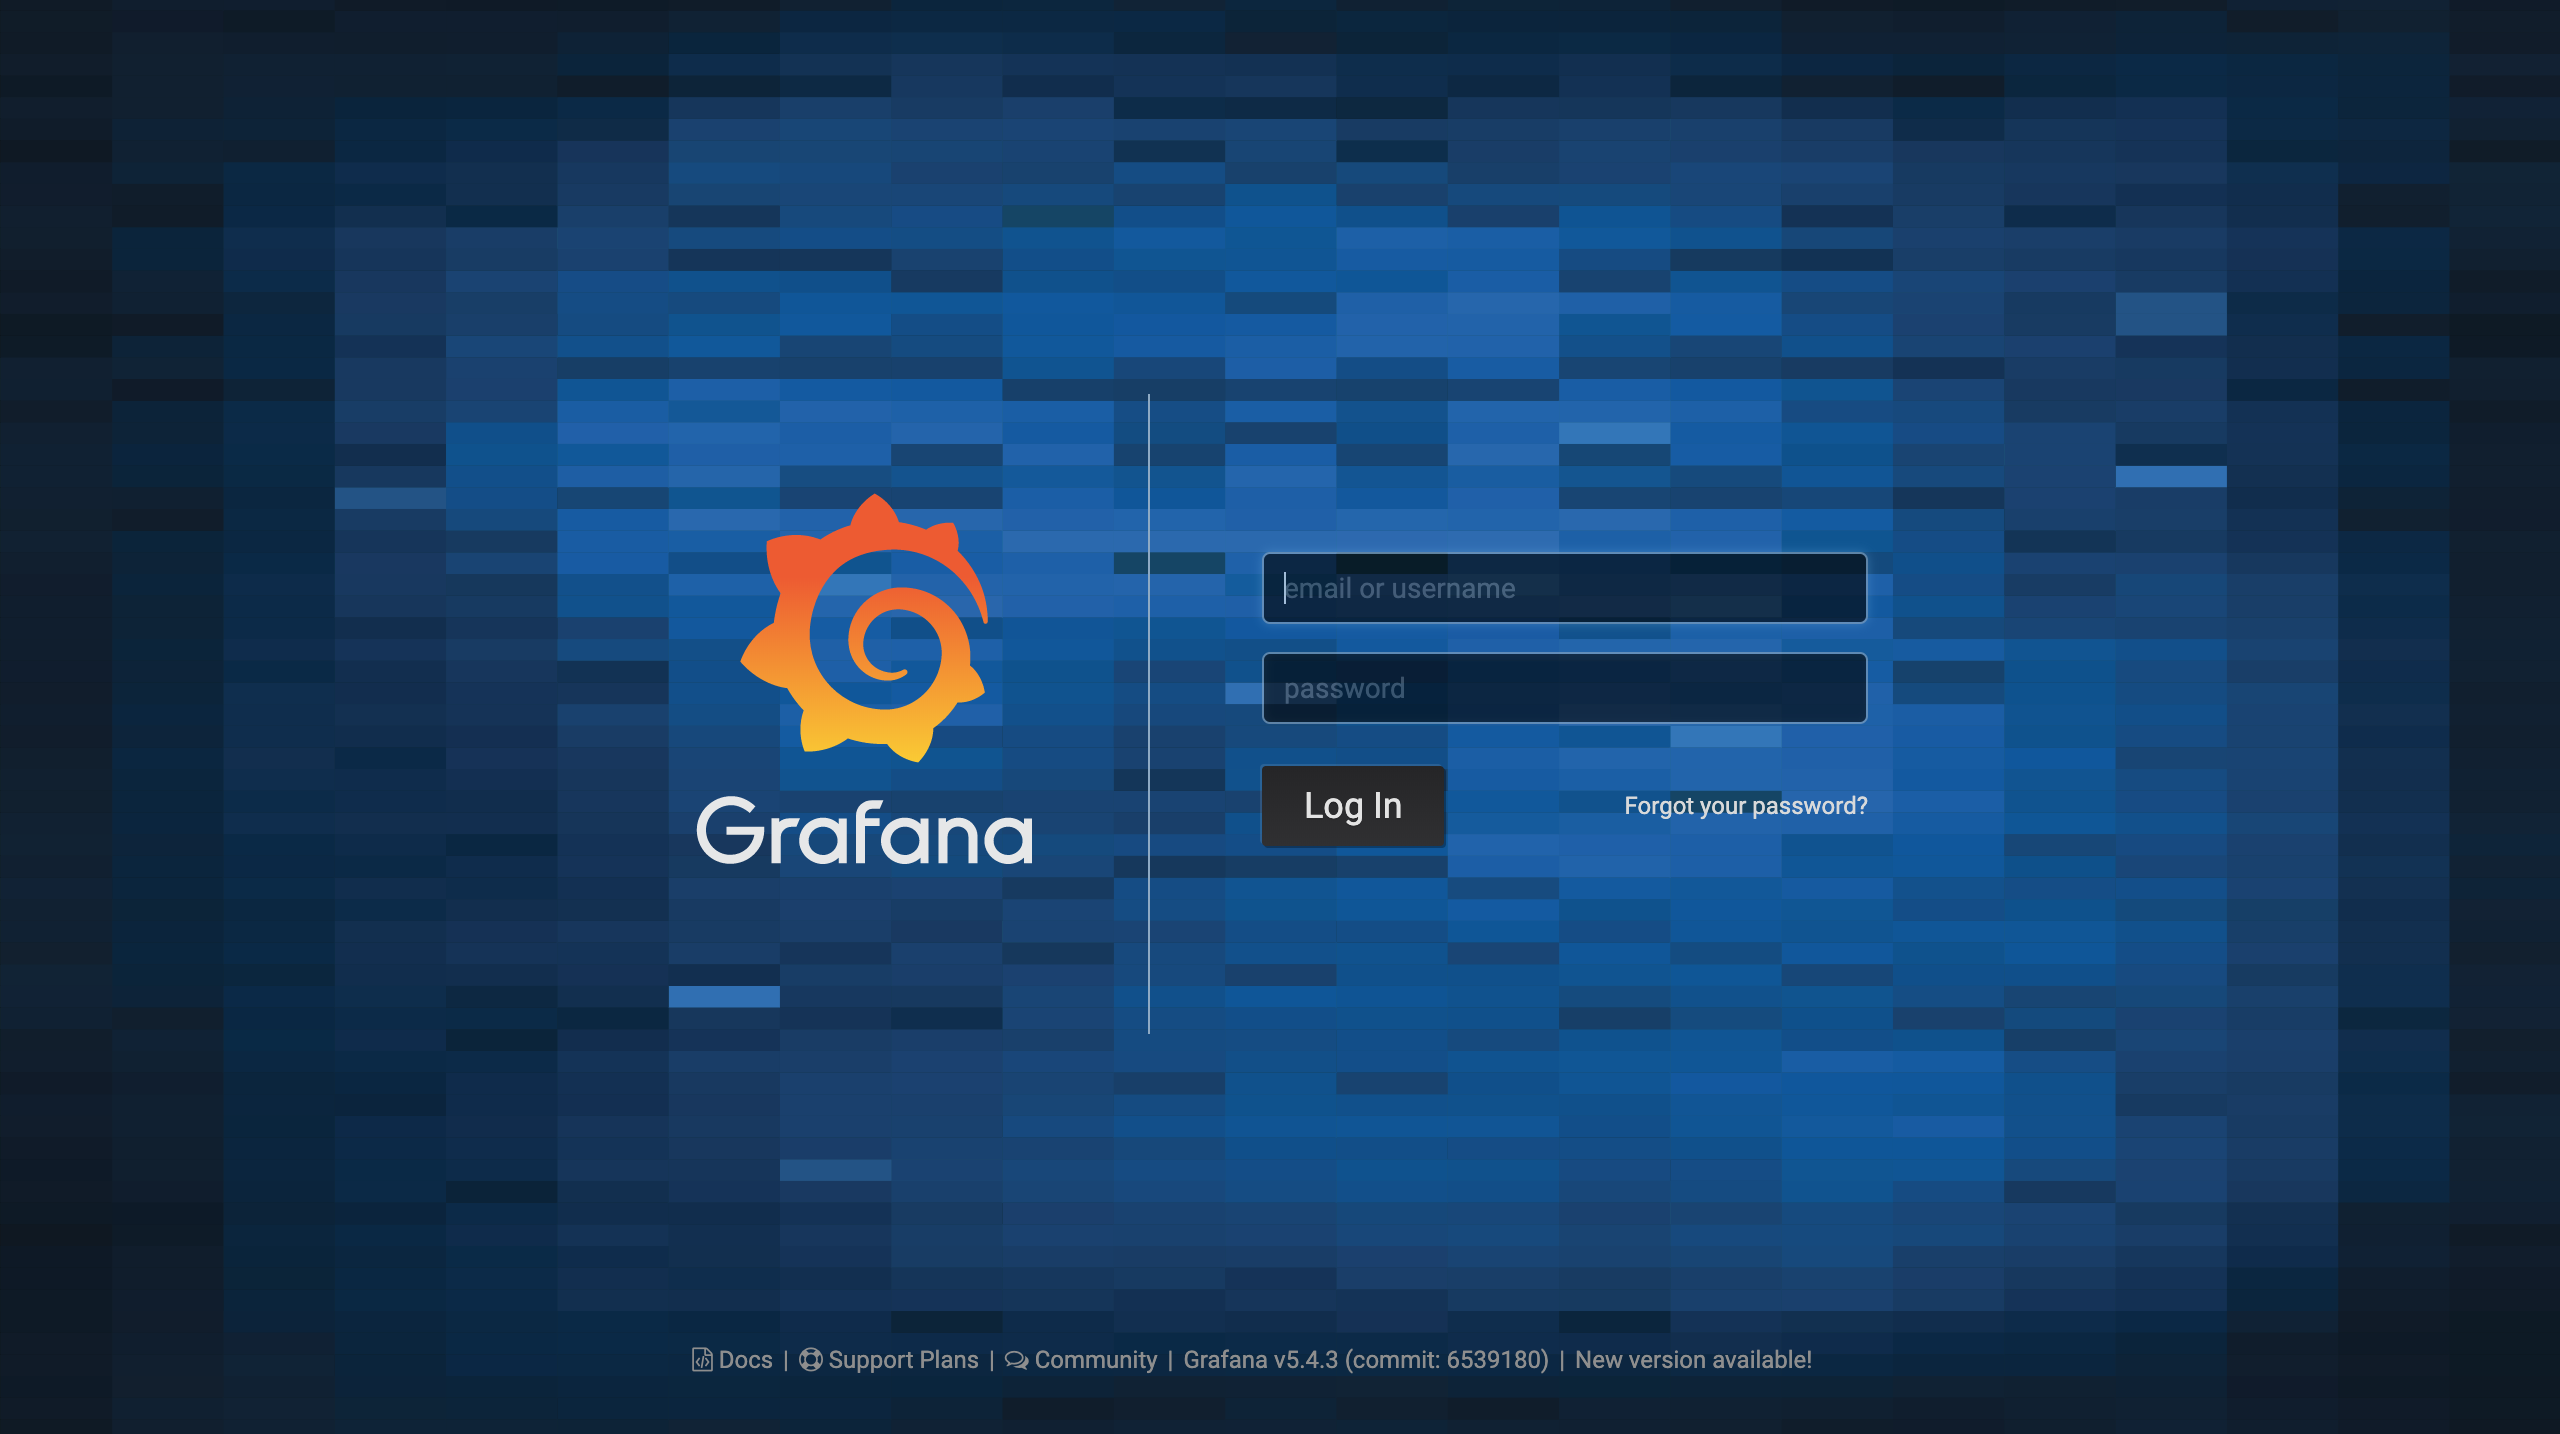
\includegraphics[scale=0.3]{./images/GrafanaLogin.png}
		 \caption{Pagina di login alla piattaforma Grafana}	
		 \label{GrafanaLogin}
	\end{center}
\end{figure}
\pagebreak

\subsection{Aggiunta Pannello alla Dashboard}\label{AddPanel}

Una volta effetuato l'accesso a \textit{Grafana} è necessario per prima cosa aggiungere alla propria Dashboard il pannello \textit{G\&B}. Gli utenti con esperienza nell'uso della piattaforma \textit{Grafana} non dovrebbero aver problemi in tal senso, ciò nonostante forniamo una descrione di questa operazione per chi ne avesse bisogno.\\

\begin{figure}[H]
	\begin{center}
		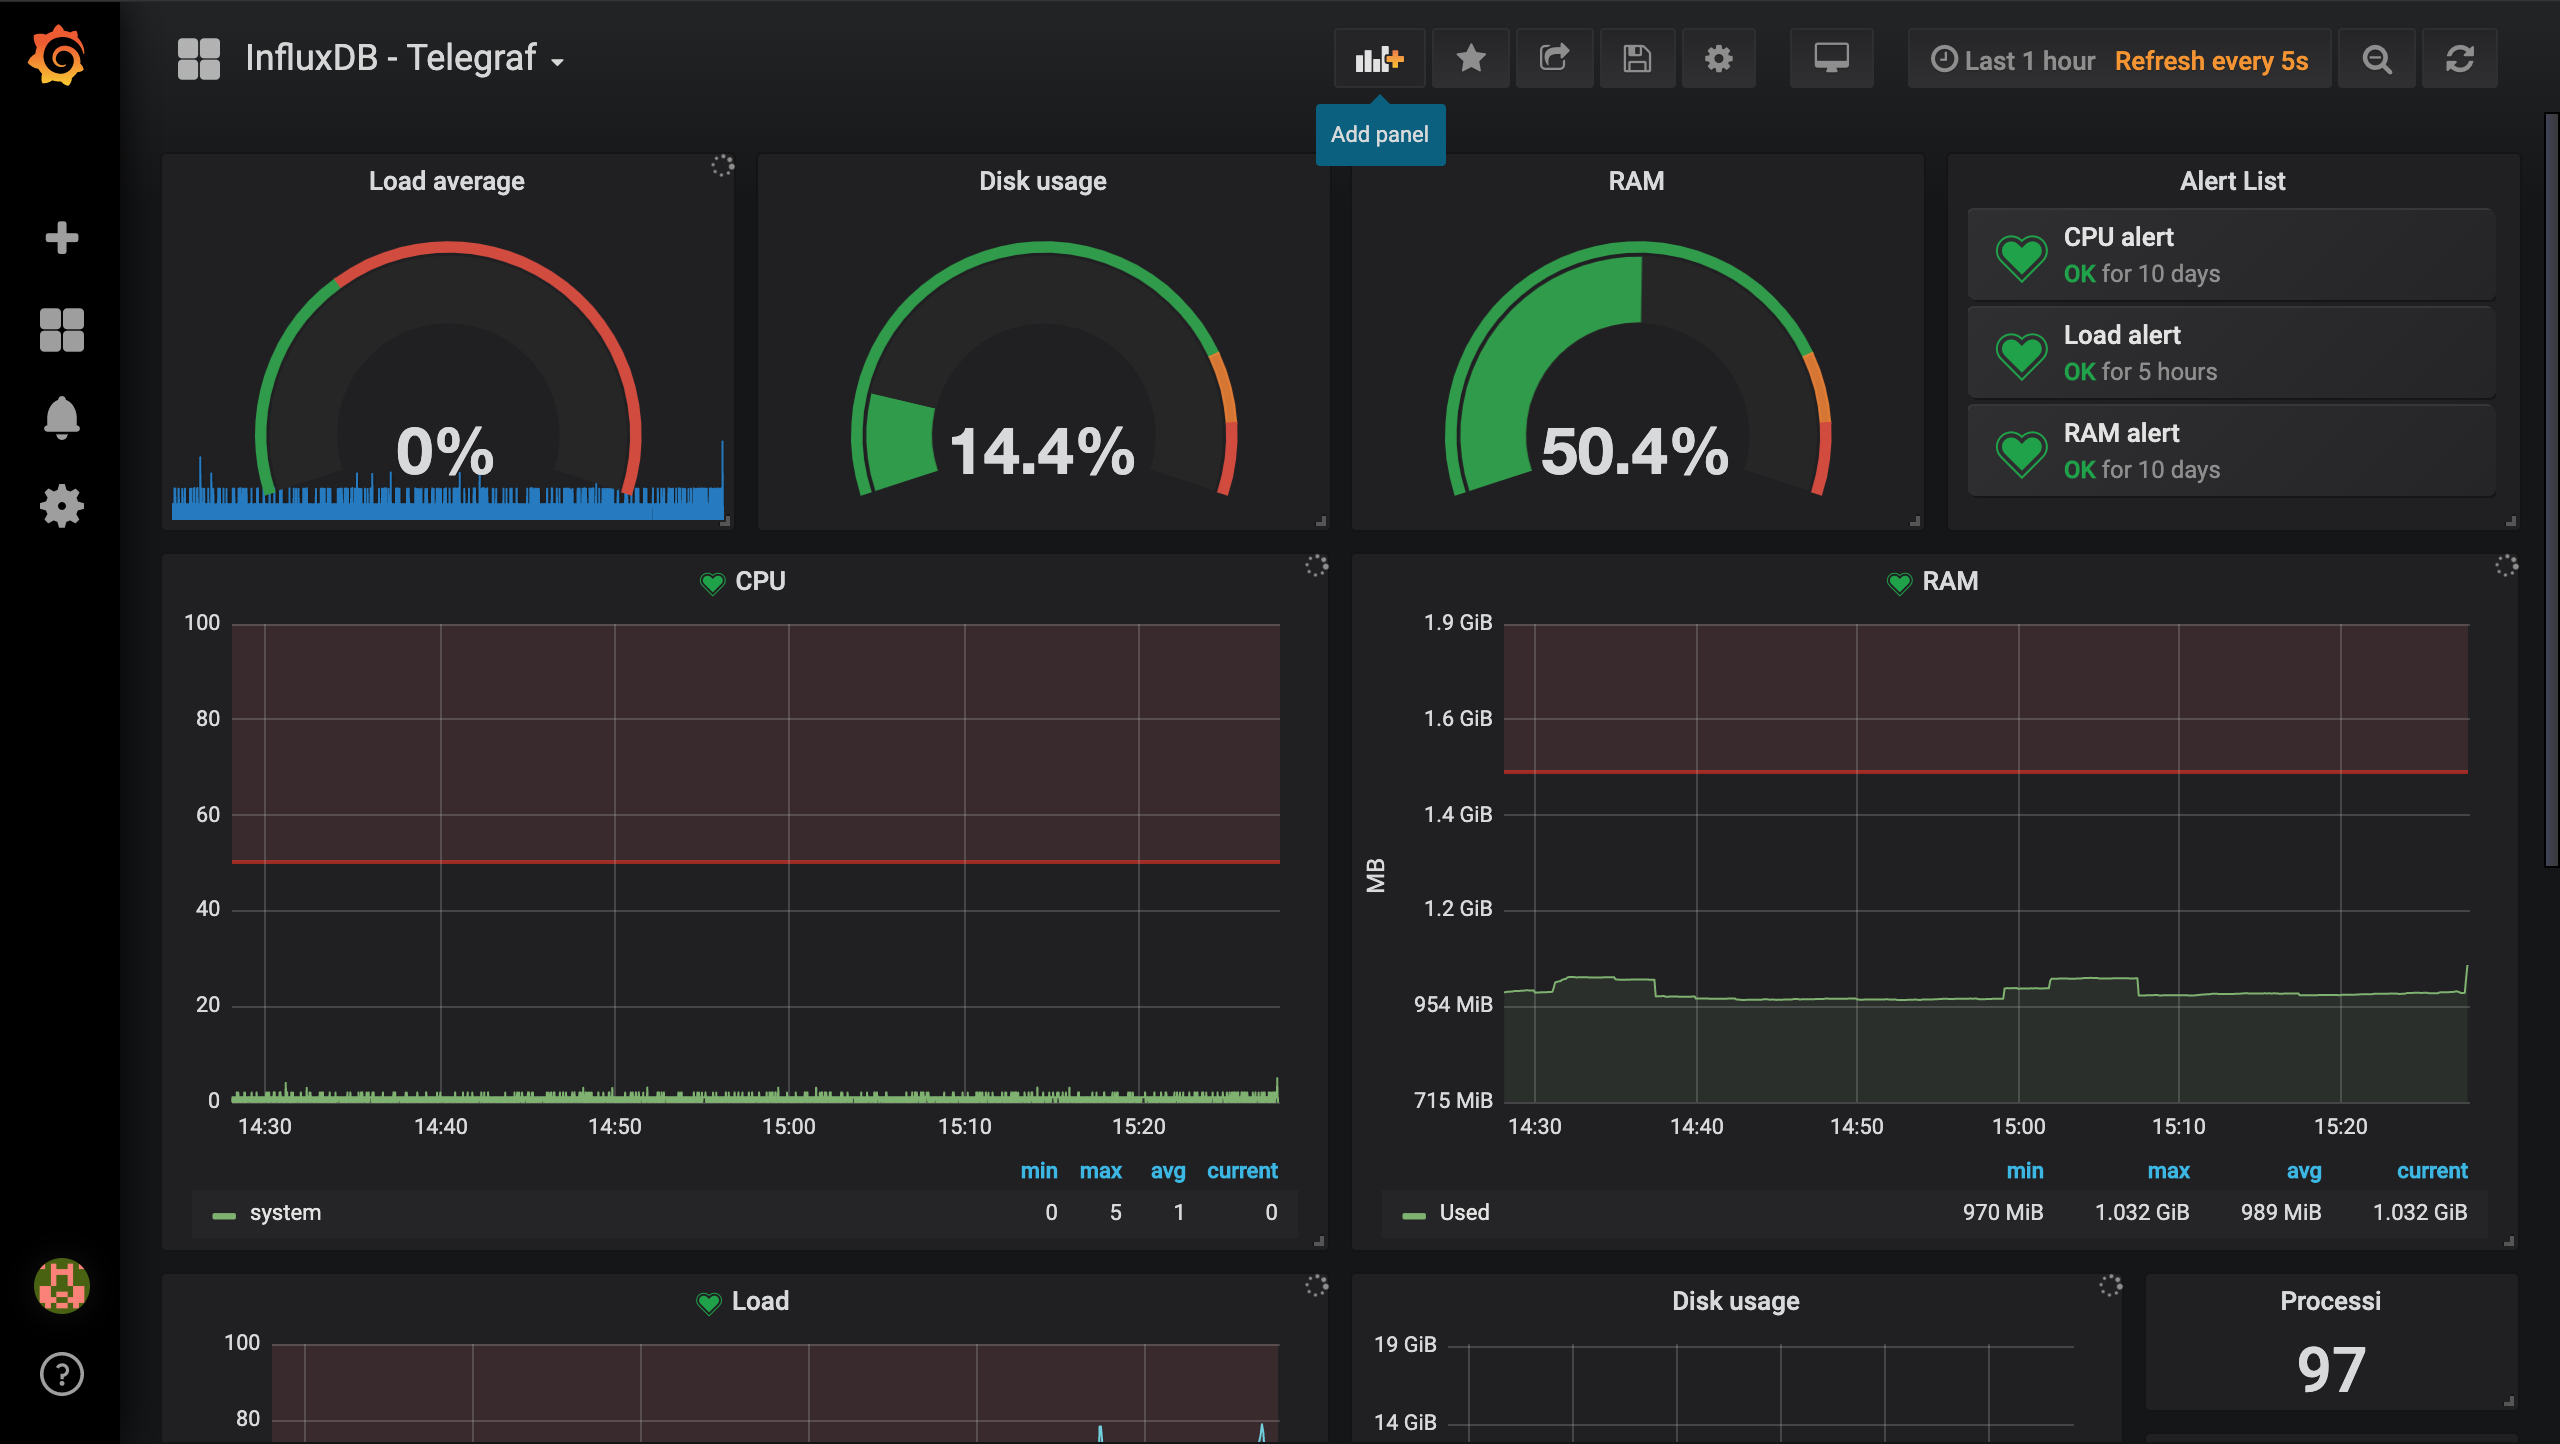
\includegraphics[scale=0.33]{./images/Dashboard.png}
		 \caption{Dashboard di esempio della piattaforma Grafana}	
		 \label{Dashboard}
	\end{center}
\end{figure}

La Figura \ref{Dashboard} espone una Dashboard di esempio, con evidenziato il dettaglio dell'hover causato dal mouse posizionato sul pulsante \textbf{Add panel}.\\
L'operazione di aggiunta del pannello si compone di due semplice passaggi:
~\\

\textbf{PASSAGGIO 1:} L'utente clicca il pulsante "Add panel" posizionato centralmente nella parte superiore della dashboard. Nella Figura \ref{Dashboard} è visibile l'effetto di hover di tale pulsante.
~\\

\textbf{PASSAGGIO 2:} L'utente,  che ora visualizza la finestra di aggiunta di un pannello, deve spostarsi nella sezione \textbf{Add} e selezionare il pannello \textit{G\&B} (Figura \ref{AddPanelImg}).

\begin{figure}[H]
	\begin{center}
		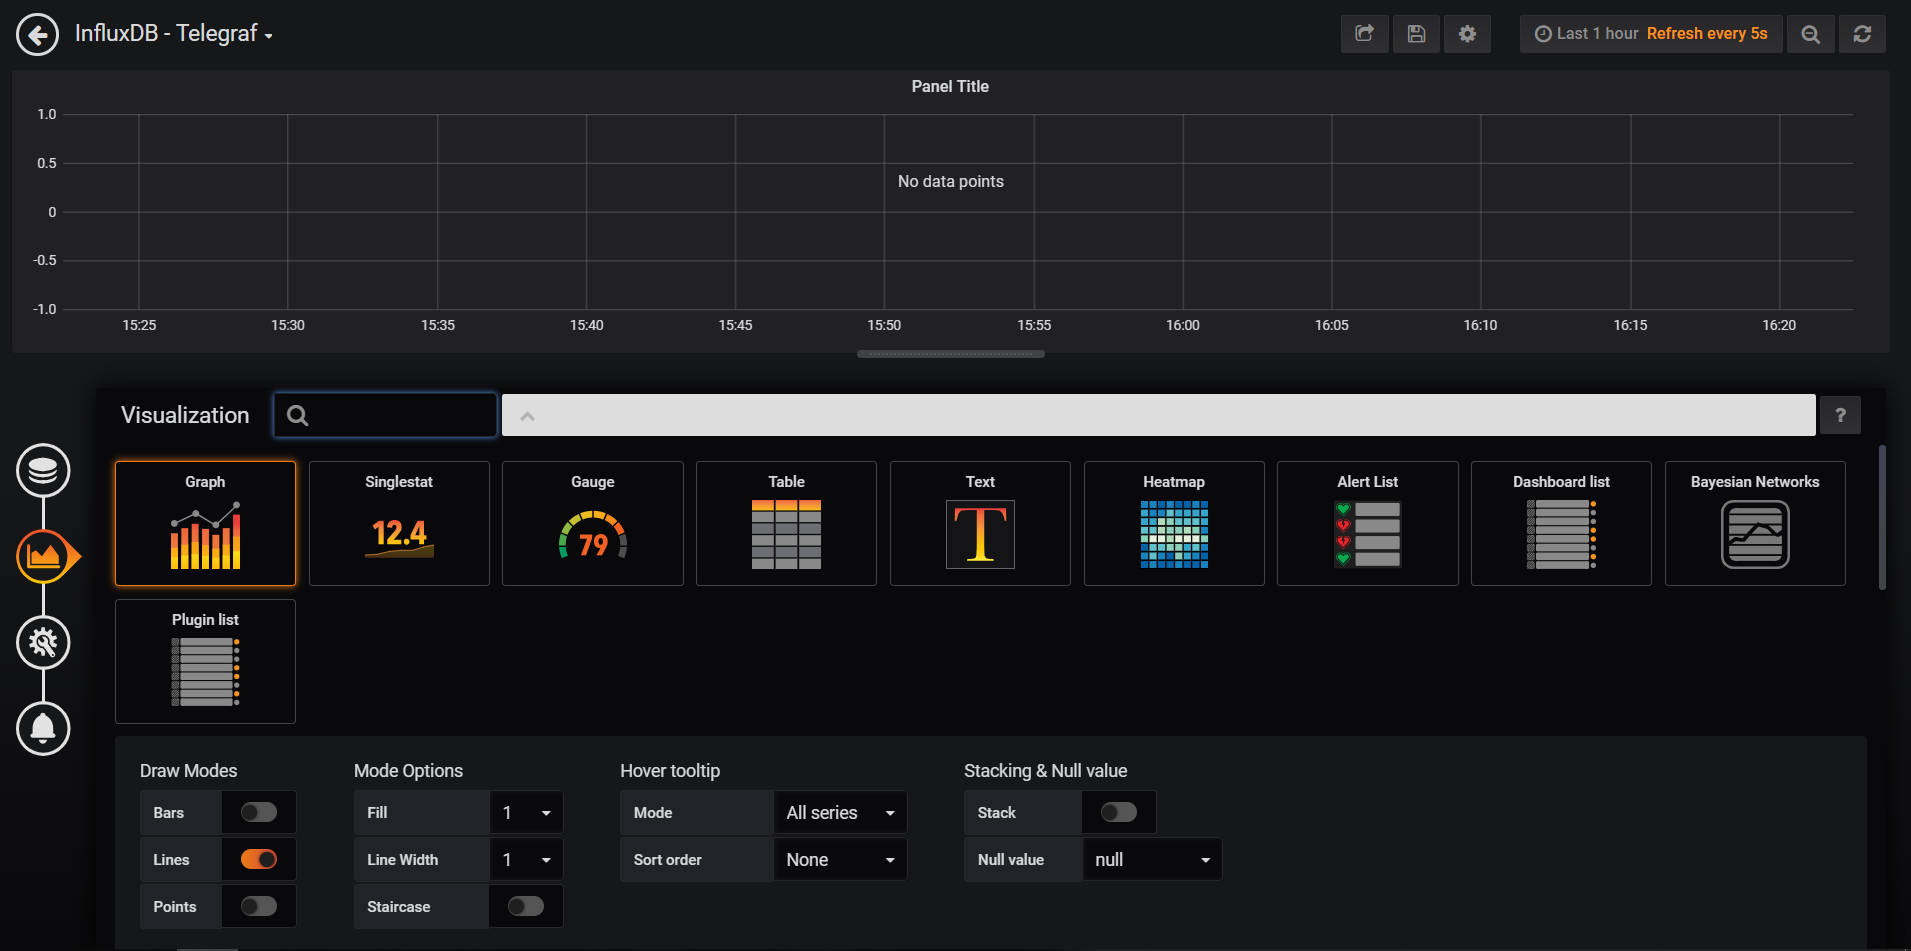
\includegraphics[scale=0.33]{./images/AddPanel.png}
		 \caption{Finestra di selezione del pannello da aggiungere alla propria Dashboard}	
		 \label{AddPanelImg}
	\end{center}
\end{figure}


Una volta selezionato il pannello sarà aggiunto alla Dashboard dell'utente, come si può vedere in Figura \ref{DashboardPanel}.

\begin{figure}[H]
	\begin{center}
		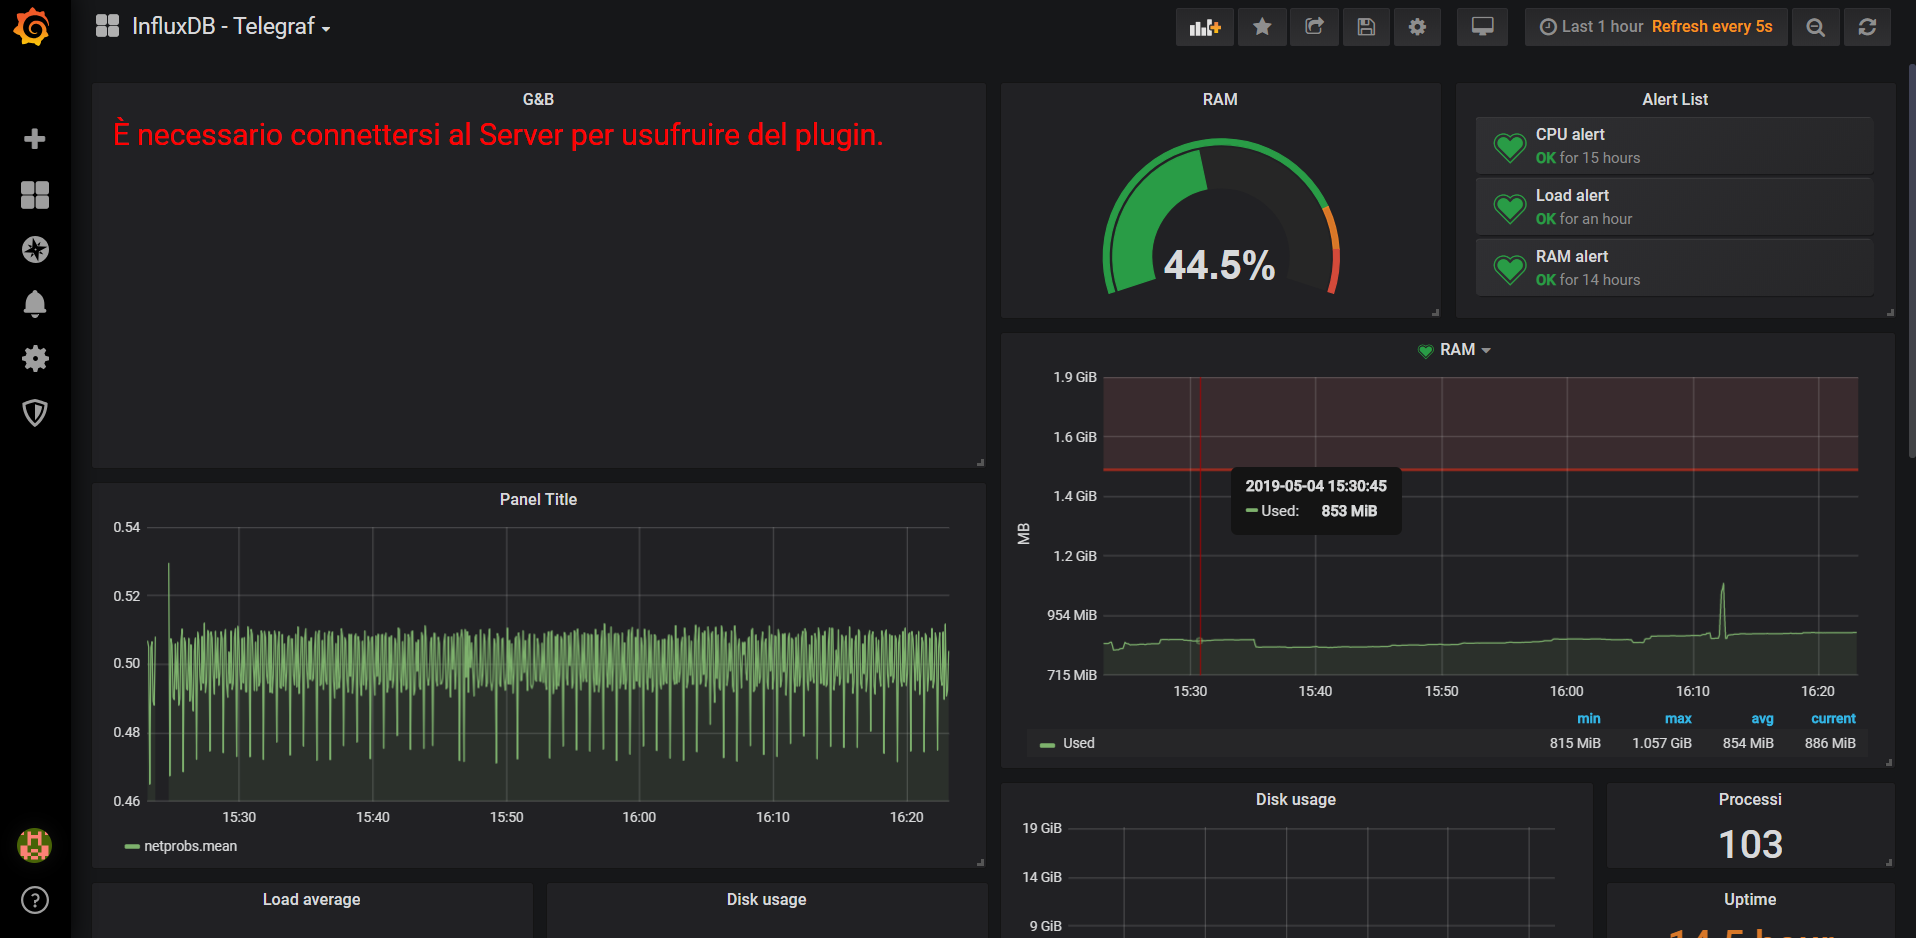
\includegraphics[scale=0.33]{./images/DashboardPanel.png}
		 \caption{Dashboard di Grafana contente il pannello G\&B}	
		 \label{DashboardPanel}
	\end{center}
\end{figure}


\pagebreak


\pagebreak

\section{Manuale d'uso}\label{Man}

\subsection{Configurazione Collegamento al Server}\label{CCS}

Una volta aggiunto alla dashboard di \textit{Grafana} il pannello \textit{G\&B} (§\ref{AddPanel}) per poter interagire in modo efficace con il pannello è necessaria, come prima operazione, configurare il collegamento al server, che è il componente che si occupa delle operazioni di ricalcolo delle probabilità. Tale operazione funge da precondizione per ogni altra funzionalità del prodotto.\\
Per poter effettuare l'operazione in esame l'utente deve innanzittuto accedere all'apposita sezione del menù di Edit del pannello, attraverso il percorso \textbf{Edit > Visualization} (Figura \ref{EditMenu}). Si ricorda che il menù di edit può essere acceduto cliccando il nome del pannello e selezionando "Edit", oppure semplicemente attraverso il click del tasto "e".

\begin{figure}[H]
	\begin{center}
		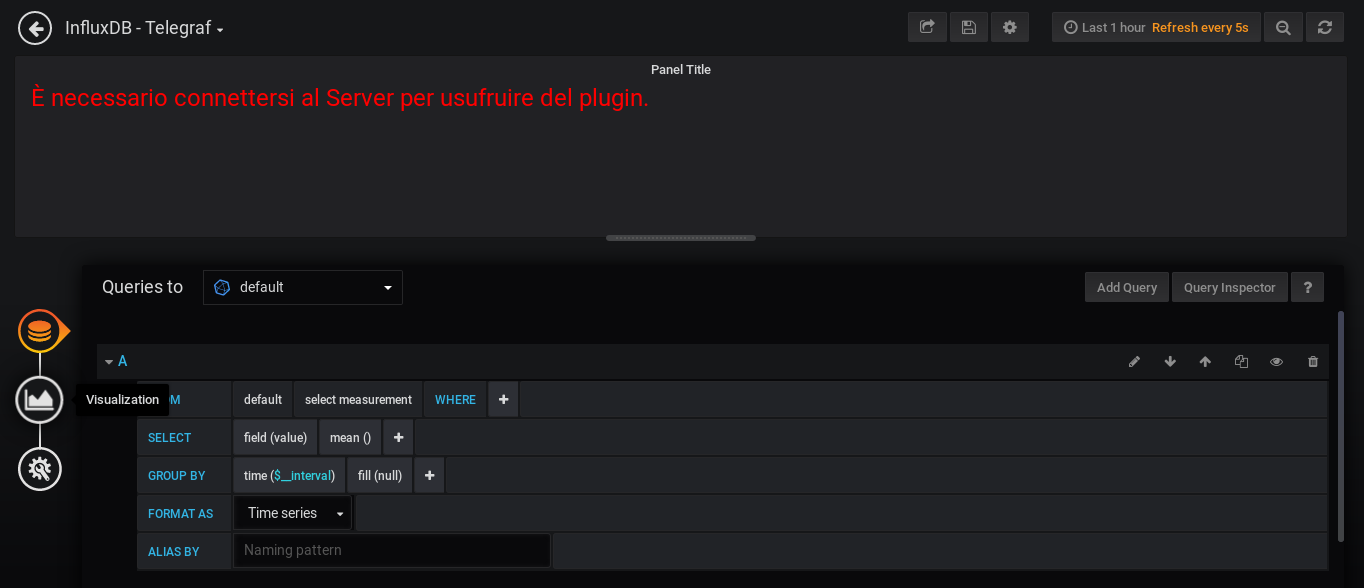
\includegraphics[scale=0.31]{./images/VisualizServerSettings.png}
		 \caption{Menù di Edit del Pannello \textit{G\&B}}	
		 \label{EditMenu}
	\end{center}
\end{figure}

Una volta selezionata la "tab" \textbf{Visualization} all'utente verrà dunque chiesto di inserire, negli appositi campi dati indicati in Figura \ref{ServerSettings}:
\begin{enumerate}
	\item Indirizzo IP del Server;
	\item Porta del Server in ascolto.
\end{enumerate}
Una volta editati i campi dati indicati l'utente deve confermare le proprie scelte premendo il pulsante \textbf{Connetti}.\\

\begin{figure}[H]
	\begin{center}
		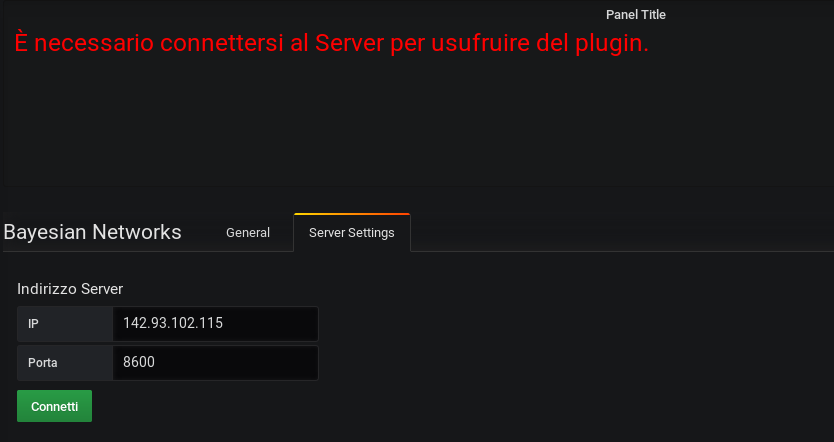
\includegraphics[scale=0.37]{./images/ServerSettings.png}
		 \caption{Sezione "Server Settings" del menù di Edit del Pannello \textit{G\&B}}	
		 \label{ServerSettings}
	\end{center}
\end{figure}

Nel caso in cui il cui la configurazione del server sia andata a buon fine l'utente viene avvisato dell'avvenuto collegamento attraverso un messaggio di notifica (Figura \ref{NotificaServer}).

\begin{figure}[H]
	\begin{center}
		
\includegraphics[scale=0.6]{./images/NotificaServer.png}
		 \caption{Notifica di avvenuto collegamento del Server}	
		 \label{NotificaServer}
	\end{center}
\end{figure}

~\\
\textbf{\textcolor{red}{ATTENZIONE}}: Nel caso in cui l'utente abbia commesso degli errori in fase di compilazione dei campi dati l'operazione non va a buon fine e l'utente viene avvisato degli errori commessi da un messaggio di errore (Figura \ref{ErroreServer}).

\begin{figure}[H]
	\begin{center}
		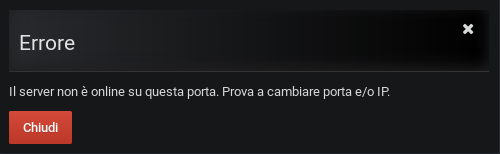
\includegraphics[scale=0.6]{./images/ErroreServer.png}
		 \caption{Messaggio di Errore configurazione Server}	
		 \label{ErroreServer}
	\end{center}
\end{figure}


Una volta configurato correttamente il collegamento al server l'utente ha accesso alla \textbf{vista principale} del plug-in:
\begin{figure}[H]
	\begin{center}
		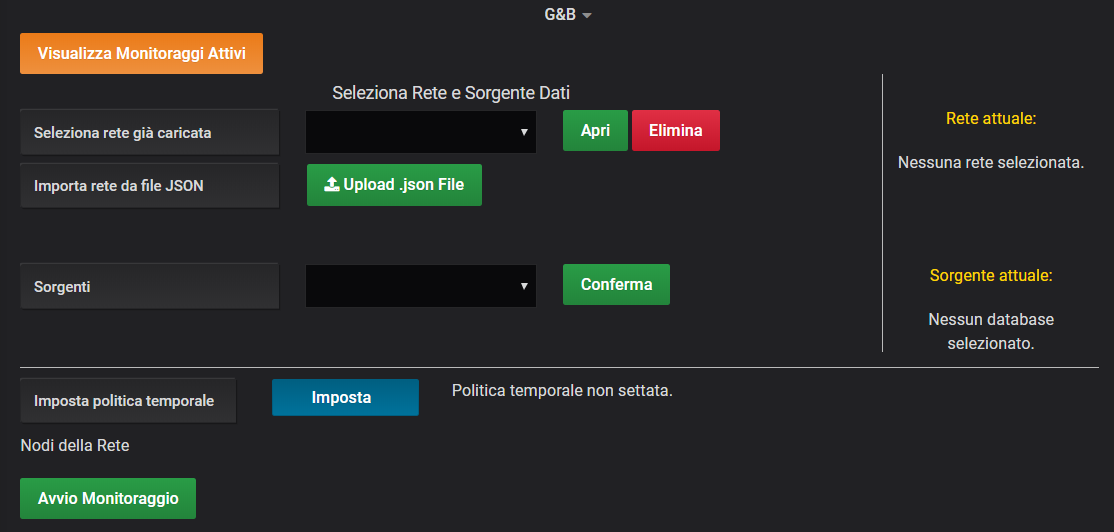
\includegraphics[scale=0.64]{./images/Panel.png}
		 \caption{Vista Principale delle Impostazioni di Collegamento del Pannello \textit{G\&B}}	
		 \label{Pannello}
	\end{center}
\end{figure}

Nello specifico la Figura \ref{Pannello} raffigura la sezione deputata alla definizione delle Impostazioni di Collegamento della rete bayesiana al flusso dati, a cui l'utente ha immediatamente accesso.


\pagebreak

\subsection{Caricamento di una Rete Bayesiana}\label{ReteB}

L'Operazione di caricamento della rete Bayesiana consta di due passaggi fondamentali:
\begin{enumerate}
	\item \textbf{Passaggio 1}: L'utente accede al pannello di selezione della rete bayesiana cliccando il pulsante \textbf{Upload .json file} presente in Figura \ref{Pannello};
	\item \textbf{Passaggio 2}: L'utente seleziona, tra i files presenti nella propria macchina, la rete bayesiana che desidera caricare e preme il pulsante \textbf{Apri} (Figura \ref{UploadRete}).
\end{enumerate} 

\begin{figure}[H]
	\begin{center}
		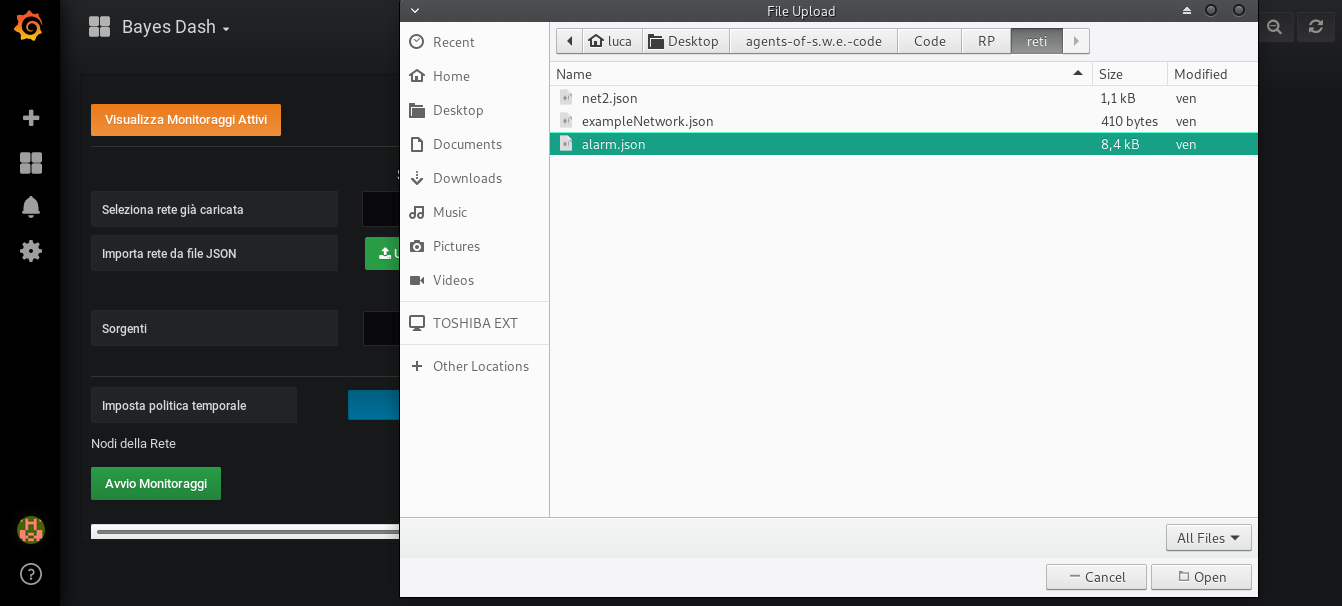
\includegraphics[scale=0.3]{./images/UpRete.png}
		 \caption{Pannello di caricamento Rete Bayesiana}	
		 \label{UploadRete}
	\end{center}
\end{figure}

L'estensione accettata dal plug-in per il file di definizione della rete è \textit{.json}. La rete bayesiana deve essere ben formata, seguendo le direttive della libreria \textit{JSBayes}. Inoltre la rete deve contenere un identificativo del proprio nominativo, necessario al momento del salvataggio della rete nel server.\\
~\\
Al seguito del corretto caricamento della rete bayesiana l'utente verrà avvisato del buon esito dell'operazione da un messaggio di notifica. Verrà inoltre visualizzato nel pannello \textit{G\&B} la lista dei nodi di cui è composta la rete bayesiana caricata (Figura \ref{NodiRete}).

\begin{figure}[H]
	\begin{center}
		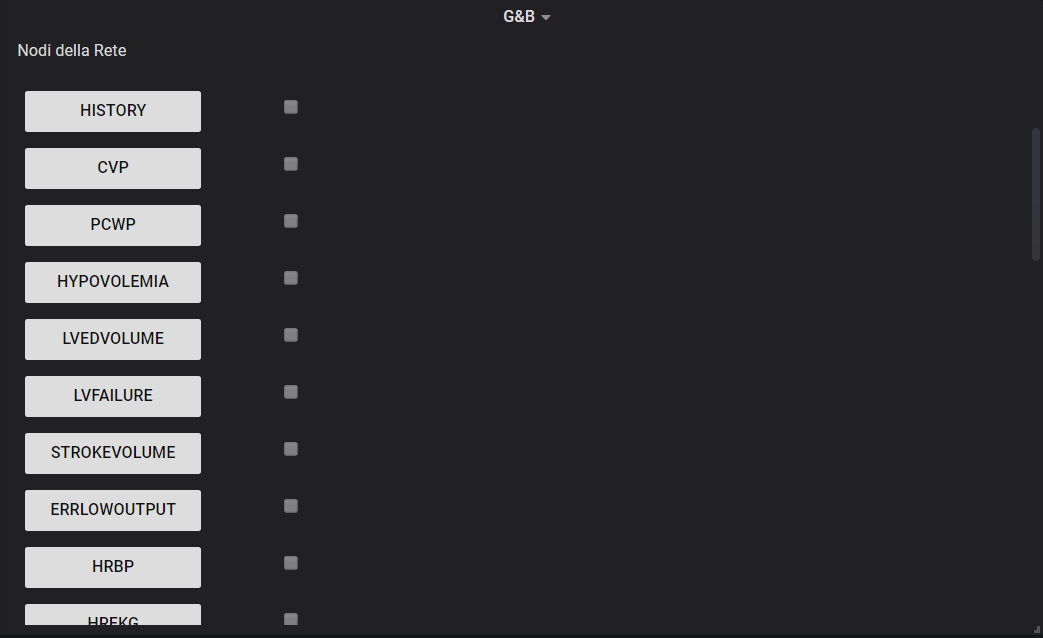
\includegraphics[scale=0.35]{./images/NodiRete.png}
		 \caption{Visualizzazione dei nodi della rete bayesiana caricata}	
		 \label{NodiRete}
	\end{center}
\end{figure}

Nel caso l'utente stesse visualizzando una diversa rete bayesiana prima del caricamento del nuovo file questa viene memorizzata nel server insieme alle sue eventuali impostazioni di collegamento.

~\\
\textbf{\textcolor{red}{ATTENZIONE}}: Nel caso in cui l'utente abbia selezionato per il caricamento un file di definizione della rete non conforme alle direttive della libreria \textit{JSBayes}, l'operazione non andrà a buon fine e l'utente verrà avvisato attraverso un apposito messagio d'errore (Figura \ref{ErroreUpRete}).

\begin{figure}[H]
	\begin{center}
		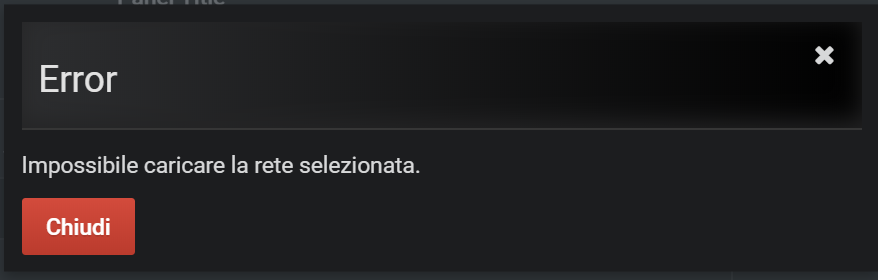
\includegraphics[scale=0.6]{./images/ErroreUpRete.png}
		 \caption{Messaggio di Errore caricamento Rete Bayesiana}	
		 \label{ErroreUpRete}
	\end{center}
\end{figure}



\pagebreak

\subsection{Selezione del Database}\label{SelectDB}

Una volta caricata una rete bayesiana (§\ref{ReteB}), al fine di collegare la stessa al flusso di monitoraggio, l'utente deve selezionare il Database contenente i dati da monitorare.\\
Tale operazione si articola in due passaggi fondamentali:
\begin{enumerate}
	\item \textbf{Passaggio 1:} L'utente seleziona, attraverso un menù a tendina, il database da usare come sorgente dati (Figura \ref{Sorgenti});
	\begin{figure}[H]
	\begin{center}
		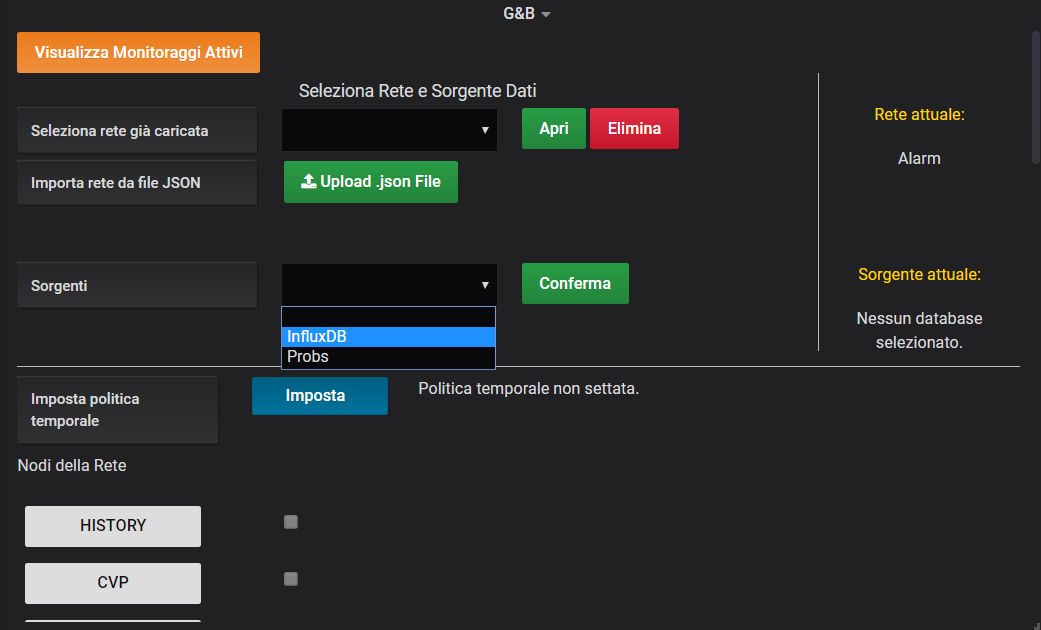
\includegraphics[scale=0.68]{./images/Sorgenti.png}
		 \caption{Elenco Database disponibili per il collegamento}	
		 \label{Sorgenti}
	\end{center}
	\end{figure}
	\item \textbf{Passagio 2:} L'utente conferma la propria scelta attraverso il pulsante \textbf{Conferma}, presente in Figura \ref{Sorgenti}.
\end{enumerate}
~\\
Al seguito della corretta selezione del Database da usare come sorgente dati l'utente verrà avvisato del buon esito dell'operazione da un messaggio di notifica (Figura \ref{NotificaSorgente}). 

\begin{figure}[H]
	\begin{center}
		
\includegraphics[scale=0.6]{./images/NotificaSorgente.png}
		 \caption{Notifica avvenuto collegamento Databse}	
		 \label{NotificaSorgente}
	\end{center}
\end{figure}

\pagebreak

\subsection{Collegamento Nodi al Flusso Dati}\label{Collegamento}

L'operazione di collegamento dei nodi della rete bayesiana al flusso dati è probabilmente la più articolata e dispendiosa del prodotto realizzato. Al fine di fornirne una spiegazione esaustiva ma al contempo intuitiva tale operazione verrà suddivisa in svariati passaggi:
~\\

\textbf{PREAMBOLO:} L'utente, a seguito del caricamento di una rete bayesiana (§\ref{ReteB}), visualizza la lista dei nodi di cui tale rete è costituita, tale situazione è presentata in Figura \ref{NodiRete}. Oltre al nominativo del nodo stesso viene visualizzata una checkbox che indica se il nodo in questione sia o meno collegato ad un flusso dati. Nel caso di nodo collegato viene visualizzato anche un pulsante \textbf{Scollega} attraverso cui è possibile scollegare il nodo dal flusso dati con un unico click.\\
Della lista di nodi visualizzata l'utente ha la possibilità di collegare ogni nodo, senza eccezioni, ad un flusso dati desiderato.
~\\

\textbf{PASSAGGIO 1:} L'utente clicca il nominativo del nodo che desidera collegare per accedere al \textbf{Pannello di Collegamento} (Figura \ref{PannelloNodo}), ove può configurare le necessarie impostazioni di collegamento per il nodo in esame.

\begin{figure}[H]
	\begin{center}
		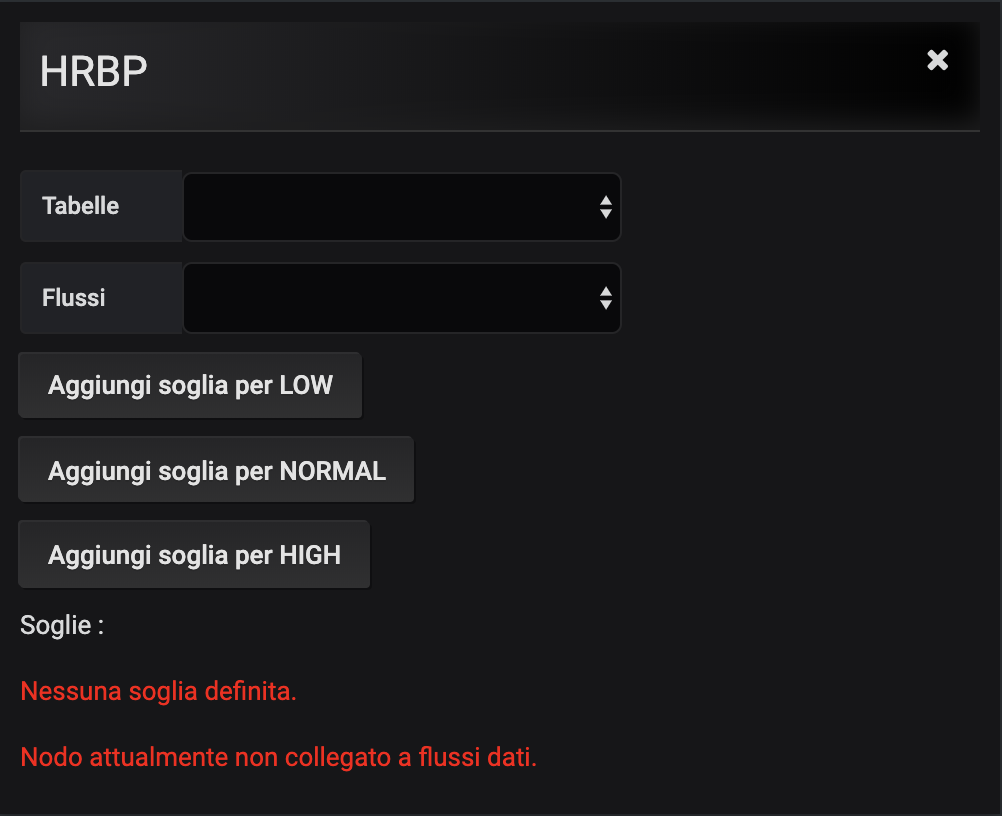
\includegraphics[scale=0.6]{./images/PannelloNodo.png}
		 \caption{Pannello di Collegamento del Nodo}	
		 \label{PannelloNodo}
	\end{center}
\end{figure}

\pagebreak

\textbf{PASSAGGIO 2:} Le prime impostazioni che l'utente è invitato a configurare riguardano la scelta della tabella, e del conseguente flusso dati (Figura \ref{PannelloNodo}), del database (selezionato in §\ref{SelectDB}). Tali impostazioni determinano univocamente lo specifico flusso dati di monitoraggio a cui l'utente collega il nodo della rete bayesiana.
~\\

\textbf{PASSAGGIO 3:} A questo punto l'utente deve configurare le soglie associate ad ogni possibile stato del nodo in esame. Tali soglie verranno verificate in sede di monitoraggio per associare un valore di evidenza al nodo della rete bayesiana in un dato istante.Possiamo suddividere questo passaggio in ultreriori cinque passi:
\begin{enumerate}
	\item L'utente seleziona \textbf{Aggiungi soglia} (pulsante presente in Figura \ref{PannelloNodo}) per aggiungere una soglia allo stato del nodo associato. È possibile aggiungere più soglie allo stesso stato;
	\item L'utente indica il valore numerico della soglia che sta definendo attraverso l'apposito campo dati visibile in Figura \ref{PannelloSoglie};
	\item L'utente seleziona, tramite la casella a scelta multipla, un valore tra i possibili: "<","<=",">" o ">=", per indicare la tipologia di soglia che sta configurando (Figura \ref{PannelloSoglie});
	\item Se lo desidera l'utente può etichettare la soglia come "critica" attraverso l'apposita checkbox (Figura \ref{PannelloSoglie}). In tal caso la verifica di tale soglia verrà fatta a prescindere dalla politica temporale delezionata in §\ref{policy};
	\item Se lo desidera l'utente può rimuovere una soglia attraverso il pulsante \textbf{Remove} presente in Figura \ref{PannelloSoglie}.
\end{enumerate}

\begin{figure}[H]
	\begin{center}
		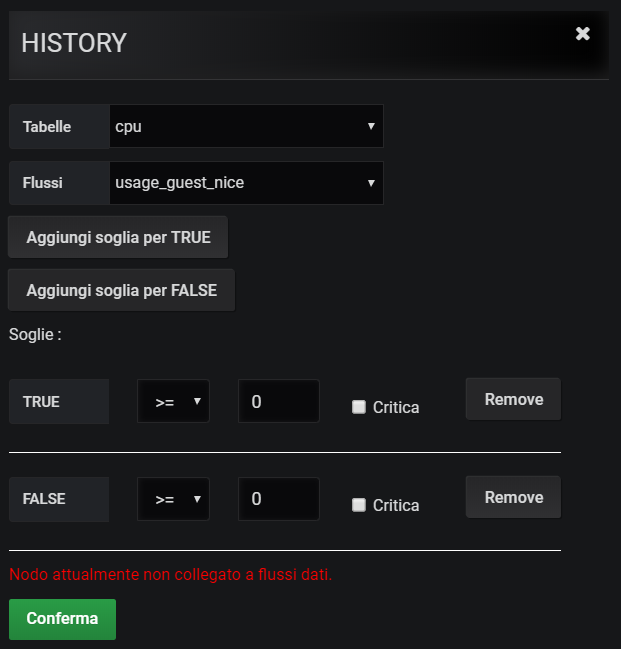
\includegraphics[scale=0.55]{./images/PannelloSoglie.png}
		 \caption{Pannello di Collegamento del Nodo con vista sulla definizione delle soglie}	
		 \label{PannelloSoglie}
	\end{center}
\end{figure}

\textbf{PASSAGGIO 4:} Infine l'utente deve confermate le proprie scelte di collegamento del nodo attraverso il pulsante \textbf{Conferma Collegamento} presente in Figura \ref{PannelloSoglie}.

~\\
A seguito del corretto collegamento del nodo al flusso dati l'utente verrà avvisato del buon esito dell'operazione da un messaggio di notifica (Figura \ref{NotificaCollegamento}).

\begin{figure}[H]
	\begin{center}
		
\includegraphics[scale=0.6]{./images/NotificaCollegamento.png}
		 \caption{Notifica di avvenuto collegamento del Nodo al flusso dati}	
		 \label{NotificaCollegamento}
	\end{center}
\end{figure}

L'utente visualizza inoltre, accanto al nodo in esame, la spunta sulla checkbox che ne indica lo stato di "Collegato al flusso dati" e il pulsante \textbf{Scollega Nodo} (Figura \ref{NodoCollegato}) per scollegare con un solo click il nodo al flusso dati.
 
 \begin{figure}[H]
	\begin{center}
		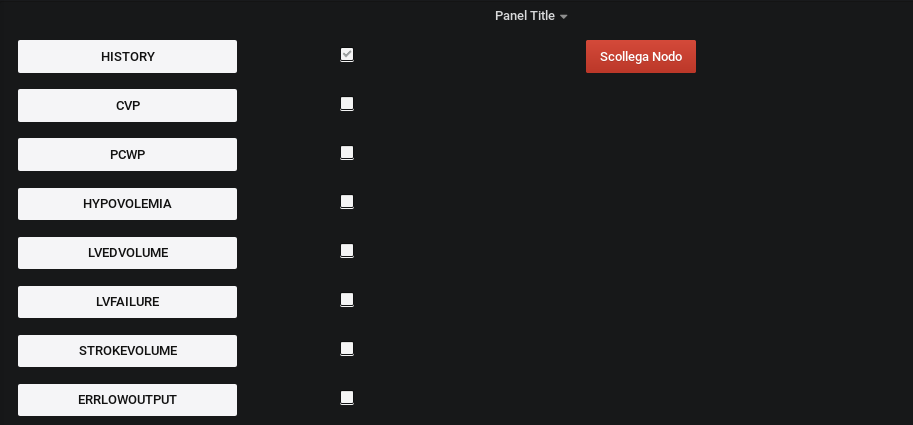
\includegraphics[scale=0.4]{./images/NodoCollegato.png}
		 \caption{Visualizzazione Nodo Collegato}	
		 \label{NodoCollegato}
	\end{center}
\end{figure}

\textbf{\textcolor{red}{ATTENZIONE}}: Nel caso in cui l'utente abbia commesso degli errori in fase di definizione delle impostazioni di collegamento l'operazione non va a buon fine e l'utente viene avvisato degli errori commessi da un messaggio di errore. Un esempio di tale situazione è fornito in Figura \ref{ErroreCollegamento}.

\begin{figure}[H]
	\begin{center}
		
\includegraphics[scale=0.6]{./images/ErroreCollegamento.png}
		 \caption{Messaggio di Errore collegamento Nodo al flusso dati}	
		 \label{ErroreCollegamento}
	\end{center}
\end{figure}
 

\pagebreak

\subsection{Definizione di una Politica Temporale di Ricalcolo}\label{policy}

L'utente deve inoltre avere la possibilità di definire un Politica Temporale per il ricalcolo delle probabilità associate ai nodi delle rete in fase di monitoraggio.\\
Per poter effettuare questa operazione l'utente deve, come prima cosa, accedere al pannello per la definizione della politica temporale tramite il pulsante \textbf{Imposta} posizionato accanto alla label "Imposta politica temporale" (Figura \ref{Pannello}).\\
~\\
L'utente deve quindi configurare la politica temporale attraverso la compilazione dei tre campi dati: "Secondi", "Minuti" ed "Ore" presenti in Figura \ref{PannelloPolicy}. Attraverso questi campi è possibile deinire con precisione e semplicità la politica temporale, ovvero il temout ciclico per il ricalcolo delle probabilità in fase di monitoraggio.

\begin{figure}[H]
	\begin{center}
		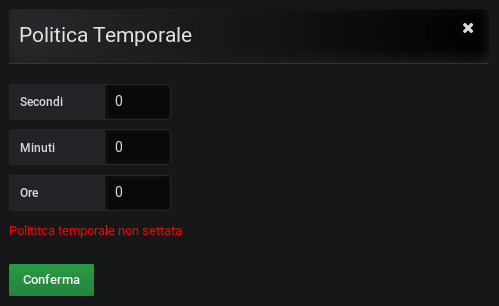
\includegraphics[scale=0.6]{./images/PannelloPolicy.png}
		 \caption{Pannello di configurazione della Politica Temporale}	
		 \label{PannelloPolicy}
	\end{center}
\end{figure} 

L'utente deve infine confermare le proprie scelte attraverso il pulsante \textbf{Conferma}, presente anch'esso in Figura \ref{PannelloPolicy}.
~\\
Al seguito della corretta definizione della politica temporale l'utente verrà avvisato del buon esito dell'operazione da un messaggio di notifica (Figura \ref{NotificaPolicy}). 

\begin{figure}[H]
	\begin{center}
		
\includegraphics[scale=0.6]{./images/NotificaPolicy.png}
		 \caption{Notifica avvenuto collegamento Databse}	
		 \label{NotificaPolicy}
	\end{center}
\end{figure}

~\\
\textbf{\textcolor{red}{ATTENZIONE}}: Nel caso in cui l'utente abbia commesso degli errori in fase di compilazione dei campi dati l'operazione non va a buon fine e l'utente viene avvisato degli errori commessi da un messaggio di errore (Figura \ref{ErrorePolicy}). Nello specifico i campi dati \textbf{"Secondi"} e \textbf{"Minuti"} accettano numeri interi compresi tra 0 e 59, mentre il campo \textbf{"Ore"} deve essere compilato con numeri interi positivi.

\begin{figure}[H]
	\begin{center}
		
\includegraphics[scale=0.6]{./images/ErrorePolicy.png}
		 \caption{Messaggio di Errore configurazione Politica Temporale}	
		 \label{ErrorePolicy}
	\end{center}
\end{figure}



\pagebreak

\subsection{Selezione di una Rete Bayesiana Esistente}\label{SelezioneRete}

Oltre a poter caricare una rete attraverso l'upload di un file di definizione in formato \textit{JSON} (§\ref{ReteB}), l'utente ha anche la possibilità di selezionare una rete già caricata in precedenza. In questo caso verranno visualizzate nel pannello \textit{G\&B} la rete selezionata con le relative impostazioni di collegamento memorizzate.\\
L'operazione di selezione di una rete bayesiana esistente si articola in due semplici passaggi:
\begin{enumerate}
	\item \textbf{Passaggio 1:} L'utente seleziona, attraverso l'apposito menù a tendina visibile in Figura \ref{SelezioneReteImg}, una delle reti bayesiane memorizzate nel server;
	\item \textbf{Passaggio 2:} L'utente conferma il caricamento cliccando il pulsante \textbf{Apri}.
\end{enumerate}

\begin{figure}[H]
	\begin{center}
		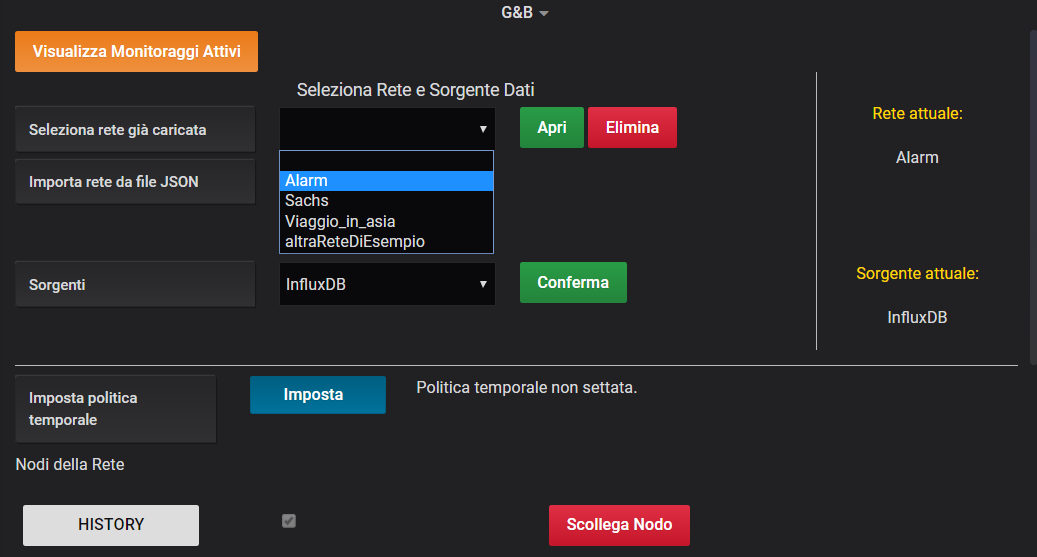
\includegraphics[scale=0.68]{./images/SelezioneRete.png}
		 \caption{Selezione di una Rete Bayesiana già Caricata}	
		 \label{SelezioneReteImg}
	\end{center}
\end{figure}

A seguito del corretto caricamento della rete bayesiana, l'utente verrà avvisato del buon esito dell'operazione da un messaggio di notifica (Figura \ref{NotificaSelezioneRete}). Inoltre, nel caso l'utente stesse visualizzando una diversa rete bayesiana prima della selezione, questa viene memorizzata nel server insieme alle sue eventuali impostazioni di collegamento.

\begin{figure}[H]
	\begin{center}
		
\includegraphics[scale=0.6]{./images/NotificaSelezioneRete.png}
		 \caption{Notifica di Avvenuto Caricamento della Rete Bayesiana}	
		 \label{NotificaSelezioneRete}
	\end{center}
\end{figure}





\pagebreak

\subsection{Eliminazione di una Rete Bayesiana}\label{EliminazioneRete}

Accanto alla selezione di una rete bayesiana già caricata (§\ref{SelezioneRete}), esiste anche l'operazione speculare di rimozione di una rete bayesiana memorizzata nel server.\\
Anche questa operazione consta di due passaggi, di cui il primo assolutamente analogo all'operazione precedente:
\begin{enumerate}
	\item \textbf{Passaggio 1:} L'utente seleziona, attraverso l'apposito menù a tendina visibile in Figura \ref{SelezioneReteImg}, una delle reti bayesiane memorizzate nel server;
	\item \textbf{Passaggio 2:} L'utente conferma l'eliminazione della rete attraverso il pulsante \textbf{Elimina}.
\end{enumerate}

A seguito della corretta rimozione della rete bayesiana, l'utente verrà avvisato del buon esito dell'operazione da un messaggio di notifica (Figura \ref{NotificaRimozioneRete}). La rete in questione, insieme alle relative impostazioni di collegamento, verrà rimossa sia dal pannello che dal server.

\begin{figure}[H]
	\begin{center}
		
\includegraphics[scale=0.6]{./images/NotificaRimozioneRete.png}
		 \caption{Notifica di Avvenuta Rimozione della Rete Bayesiana}	
		 \label{NotificaRimozioneRete}
	\end{center}
\end{figure}

\textbf{\textcolor{red}{ATTENZIONE}}: Nel caso in cui l'utente abbia scelto di eliminare una rete al momento sotto monitoraggio attivo l'operazione non va a buon fine e l'utente viene avvisato di tale risultato da un messaggio di errore (Figura \ref{ErroreDeleteNet}).

\begin{figure}[H]
	\begin{center}
		
\includegraphics[scale=0.6]{./images/ErroreDeleteNet.png}
		 \caption{Messaggio di Errore Eliminazione di una Rete Bayesiana}	
		 \label{ErroreDeleteNet}
	\end{center}
\end{figure}


\pagebreak

\subsection{Avvio Monitoraggio}\label{Avvio}

L'utente ha la possibilità di avviare il monitoraggio della rete bayesiana visualizzata al momento sul pannello \textit{G\&B} attraverso il pulsante \textbf{Avvio Monitoraggio} come si vede in Figura \ref{AvvioMonitoraggio}.

\begin{figure}[H]
	\begin{center}
		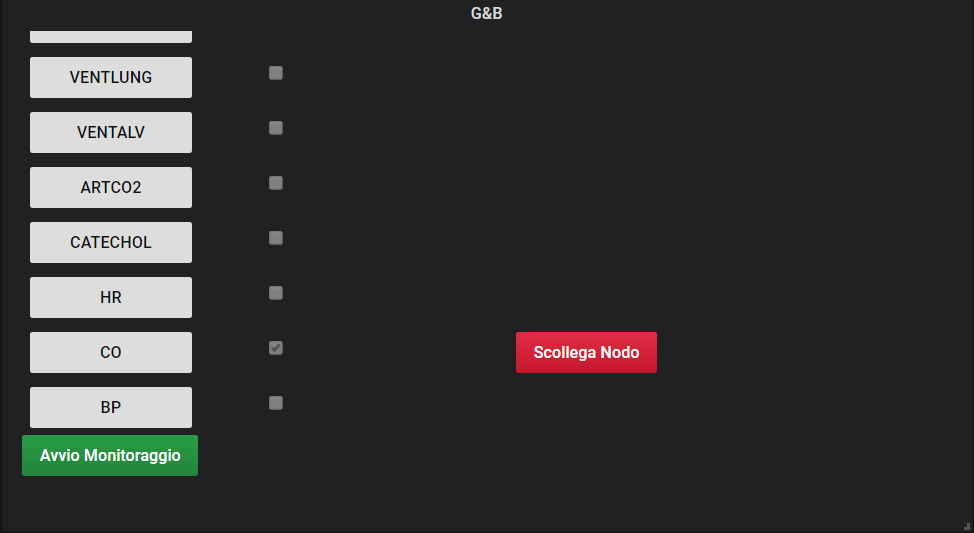
\includegraphics[scale=0.4]{./images/AvvioMonitoraggio.png}
		 \caption{Vista dell'Avvio del Monitoraggio}	
		 \label{AvvioMonitoraggio}
	\end{center}
\end{figure}

Affinchè il monitoraggio della rete possa essere avviato correttamente è necessario che l'utente abbia in precedenza completato tutte le necessarie operazioni di configurazione del collegamento della rete bayesiana al flusso di monitoraggio.\\
Nello specifico è necessario che l'utente, oltre ovviamente ad aver caricato una rete bayesiana (§\ref{ReteB}), deve aver:
\begin{itemize}
	\item Selezionato un database da usare come sorgente dei dati di monitoraggio (§\ref{SelectDB});
	\item Definito una politica temporale per il ricalcolo delle probabilità (§\ref{policy});
	\item Collegato almeno un nodo durante §\ref{Collegamento}.
\end{itemize} 

\pagebreak

\textbf{\textcolor{red}{ATTENZIONE}}: Nel caso in cui l'utente non abbia correttamente completato una delle operazioni precedentemente elencate il monitoraggio della rete non viene avviato e l'utente viene avvisato degli errori commessi da un messaggio di errore (Figura \ref{ErroreAvvio}).

\begin{figure}[H]
	\begin{center}
		
\includegraphics[scale=0.6]{./images/ErroreAvvio.png}
		 \caption{Messaggio di Errore Avvio Monitoraggio}	
		 \label{ErroreAvvio}
	\end{center}
\end{figure}

Nel caso in cui il cui, invece, l'avvio del monitoraggio dati sia andato a buon fine l'utente viene avvisato del buon esito dell'operazione attraverso un messaggio di notifica (Figura \ref{NotificaMonitoraggio}). La rete bayesiana, con le relative impostazioni di collegamento, viene inviata al server, il quale la memorizza e comincia ad eseguire le necessarie operazioni di ricalcolo delle probabilità per fornire all'utente dati di monitoraggio in tempo reale.

\begin{figure}[H]
	\begin{center}
		
\includegraphics[scale=0.6]{./images/NotificaMonitoraggio.png}
		 \caption{Notifica di Avvio Monitoraggio Dati}	
		 \label{NotificaMonitoraggio}
	\end{center}
\end{figure}




\pagebreak

\subsection{Visualizzazione Monitoraggi Attivi}\label{MonitoraggiAttivi}

Una volta avviato il monitoraggio (§\ref{Avvio}), per visualizzare effitavamente in tempo reali i dati di monitoraggio, è necessario innanzitutto accedere alla sezione per la visualizzazione dei Monitoraggi Attivi.\\
L'utente può accedere in ogni momento alla visualizzazione dei Monitoraggi attivi attraverso il pulsante \textbf{Visualizza Monitoraggi Attivi} posizionato in alto a sinistra nella vista principale del pannello, come si può vedere in Figura \ref{Pannello}.\\

Accedere alla sezione dei Monitoraggi Attivi porta alla scomparsa della precedente vista del pannello, che è infatti unicamente dedicata alle operazioni di configurazione delle impostazioni di collegamento della reta al flusso dati.


\subsection{Visualizzazione Impostazioni di Collegamento}\label{ImpostazioniCollegamento}

L'utente, quando si trova nella sezione del pannello dedicata alla visualizzazione dei monitoraggi attivi, può in ogni momento tornare alla parte dedicata alla configurazione delle impostazioni di collegamento attraverso il pulsante \textbf{Visualizza Impostazioni} (Figura \ref{VisualizzaImpostazioni})\\

\begin{figure}[H]
	\begin{center}
		
\includegraphics[scale=0.6]{./images/VisualizzaImpostazioni.png}
		 \caption{Pulsante per la Visualizzazione delle Impostazioni di Collegamento}	
		 \label{VisualizzaImpostazioni}
	\end{center}
\end{figure}



\pagebreak

\subsection{Interruzione Monitoraggio}\label{Interruzioe}

\pagebreak

\subsection{Visualizzazione Dati di Monitoraggio}\label{VisualDati}




\pagebreak

\section{FAQ}\label{FAQ}


\subsection*{1 Non vedo il pannello G\&B. Dov'è?}
Una volta eseguito l'accesso a \textit{Grafana} è necessario aggiungere il pannello \textit{G\&B} alla propria dashboard per poter usufruire delle sue funzionalità. In tal senso l'operazione necessaria è descitta nel dettaglio in questa sezione: §\ref{AddPanel}.

\subsection*{2 Non riesco a collegare il Server. Perchè?}
Il server è una componente necessaria al corretto funzionamento del plug-in \textit{G\&B}, senza di esso il pannello non può funzionare correttamente. Per poter effettuare con successo il collegamento è necessario avere un server attivo, con una porta aperta in ascolto. Per tutti i dettagli necessari vi invitiamo a consultare l'apposita sezione: \ref{Server}.

\subsection*{3 Non riesco a caricare la rete bayesiana e non capisco gli errori che mi vengono segnalati. Cosa devo fare?}
L'operazione di caricamento di una rete bayesiana attraverso il file di definizione in formato \textit{JSON}, descritta in §\ref{ReteB}, può fallire solamente nel caso in cui il file caricato non contenga una rete ben formata.\\
Per garantire il corretto funzionamento del prodotto è infatti necessario che la rete bayesiana definita nel file \textit{JSON} abbia una struttura specifica, conforme alle specifiche definite in \ref{strutturaRete}. Nel caso in cui gli errori segnalati dal sistema in fase di caricamento non fossero adeguatamente autoesplicativi per la comprensione del problema vi invitiamo a consultare la sezione §\ref{strutturaRete}, in cui viene spiegato nel dettaglio come deve essere strutturata la rete bayesiana.

\subsection*{4 Durante il collegamento di un nodo i menù a tendina per la selezione della tabella e del flusso dati sono vuote. Cosa devo fare?}
Prima di procedere con l'operazione di collegamento dei nodi (§\ref{Collegamento}) assicuratevi sempre di aver prima selezionato un Database da usare come sorgente dei dati. Tale operazione è descritta nella sezione §\ref{SelectDB} ed influenza la possibile scelta di tabella e flusso dati durante il collegamento dei nodi. Nel caso in cui non sia selezionato alcun database non vi sarà alcuna possibile scelta di tabella e flussi durante il collegamento dei nodi.

\subsection*{5 Quanti/Quali nodi devo collegare per avviare il monitoraggio della rete?}
La risposta a questa domanda non è univoca, dipende quasi totalemente dalla struttura della rete bayesiana in questione. Nel caso la rete sia stata fornita da un esperto vi consigliamo in ogni caso di chiedere all'ideatore della rete. In caso contrario sappiate che non esiste un numero "corretto" di nodi da collegare, possiamo però fornirvi alcune \textbf{raccomandazioni} di carattere generale in merito a quanti e/o quali nodi andrebbero collegati:
\begin{itemize}
	\item Ovviamente è necessario collegare almeno un nodo al flusso dati, altrimenti il sistema non consente neppure di avviare il monitoraggio;
	\item Collegare tutti i nodi della rete al flusso non ha senso. L'utilità di sfruttare le reti bayesiane per il monitoraggio dei dati infatti sta tutto nel poter ricevere dati in merito a nodi non collegati al flusso, attraverso il monitoraggio di nodi a loro collegati nella struttura della rete.
	\item Idealmente tutti i nodi che rappresentano condizioni immediatamente ricavabili dal flusso dati andrebbero collegati. I nodi da non collegare dovrebbero essere solo quelli il cui stato non può essere osservato immediatamente dai dati.
\end{itemize}

\subsection*{6 Devo definire una soglia per ogni stato del nodo durante il collegamento?}
No, non è necessario. Affinchè il collegamento di un nodo possa essere confermato con successo è sufficiente che venga definita una sola soglia. Nel caso in cui i valori monitorati non comportino il superamento di alcuna soglia per un dato nodo le probabilità associate ai suoi stati verranno infatti valutate sulla base delle informazioni della rete bayesiana in questione.\\
Tuttavia, per modellare con maggior precisione ogni possibile situazione, \textbf{consigliamo} di associare almeno una soglia per ogni stato di ogni nodo collegato al flusso dati.

\subsection*{7 Quando devo etichettare una soglia come critica? Qaunte ne devo definire?}
Durante l'operazione di collegamento dei nodi al flusso dati, descritta nella sezione §\ref{Collegamento}, l'utente ha la possibilità, nel definire le soglie del nodo, di indicarne una o più come "critiche". Questa è una funzionalità potente, che deve essere ben gestita da parte dell'utente.\\
Le soglie critiche dovrebbero essere usate \textbf{solo} per il controllo di condizioni \textbf{straordinarie} che, nel caso si verifichino durante il monitoraggio, richiederebbero un immediato ricalcolo delle probabilità, senza l'attesa della scadenza del timer definito dalla politica temporale.\\
Un numero di soglie critiche troppo elevato, oppure la definizione di soglie critiche troppo facilmente verificabili, comporterebbe un ricalcolo delle probabilità troppo frequente, andando inoltre a svilire e rendere inutile la definizione della politica temporale per il ricalcolo delle probabilità (§\ref{policy}).\\
Di conseguenza non vi è un numero corretto di soglie critiche da definire, tuttavia raccomandiamo caldamente di definirne un numero contenuto, e di usarle unicamente per modellare condizioni straordinarie di cui si vuole essere aggiornati in tempo reale.

\subsection*{8 Che politica temporale devo impostare?}
Nuovamente, come nella domanda precedente, nel caso in cui sia stato un esperto a fornirvi la rete bayesiana consigliamo sempre di domandare a lui. In caso contrario dipende dalla rete in questione e dalla tipologia di dati che desiderate monitorare.\\
Politiche temporali troppo brevi potrebbero portarvi ad un sovraccarico nel caso in cui la vostra rete fosse particolarmente ricca di nodi, occorre inoltre valutare, soprattutto per la visualizzazione dei dati di monitoraggio (§\ref{VisualDati}) che la piattaforma \textit{Grafana} consente il refresh dei dati della pagina a intervalli prestabiliti, in ogni caso non inferiori ai 5 secondi. D'altro canto politiche temporali troppo lunghe potrebbero essere scarsamente utili, soprattutto nel caso in cui non aveste definito correttamente soglie critiche durante l'operazione di collegamento dei nodi (§\ref{Collegamento}).\\
Di conseguenza consigliamo una politica temporale moderata, in base alla tipologia di dati in questione. Nel caso in cui temeste di non aver sufficiente tempestività nel ricalcolo delle probabilità vi invitiamo a mantenere una politica moderata definendo correttamente alcune soglie critiche durante il collegamento dei nodi.

\subsection*{9 I dati di monitoraggio derivati da una rete che ho collegato non vengono aggiornati in base a quanto ho definito nella politica temporale. Perchè?}
La politica temporale che viene impostata dall'utente (operazione definita nella sezione §\ref{policy}) influenza unicamente il ricalcolo delle probabilità eseguito dal server. La \textbf{visualizzazione} di tali dati aggiornati dipende dal timer di refresh della pagina, impostazione propria di \textit{Grafana}.\\
Invitiamo duqnue l'utente a definire, attraverso le impostazioni proprie di \textit{Grafana}, un timer per il refresh della pagina che sia quantomeno pari a quello definito dalla politica temporale, oppure a far si che la politica temporale sia un multiplo del refreh della pagina di \textit{Grafana}.\\

\subsection*{10 Come faccio a definire alert basati sui dati di monitoraggio?}
La definizione di alert è un'operazione propria della piattaforma \textit{Grafana}, non è dunque collegata direttamente al pannello \textit{G\&B}. Tuttavia l'utente può ovviamente definire alert sui dati di monitoraggio rilevati dal sistema.\\
Nello specifico, attraverso le funzionalità messe a disposizione da \textit{Grafana}, l'utente deve creare un pannello grafico basato sui dati di monitoraggio e definirvi sopra gli alert desiderati.\\
Ricordiamo che il monitoraggio dei dati è costante e indipendente dal pannello, grazie all'uso del server per il ricalcolo delle probabilità. Non è dunque necessario che il pannello \textit{G\&B} sia presente nella dashboard dell'utente affinchè gli alert definiti su monitoraggi attivi vengano costantemente aggiornati.



\pagebreak

\section{Segnalazione Errori e Malfunzionamenti}\label{Segnalazione}

\pagebreak

\appendix
\section{Struttura del File JSON per la Definizione di una Rete Bayesiana}\label{strutturaRete}

Questa sezione ha lo scopo di spiegare all'utente il corretto modo di definire il file \textit{.JSON} per la definizione della rete bayesiana da importare nel plug-in e successivamente utilizzala.


\begin{figure}[H]
	\begin{center}
		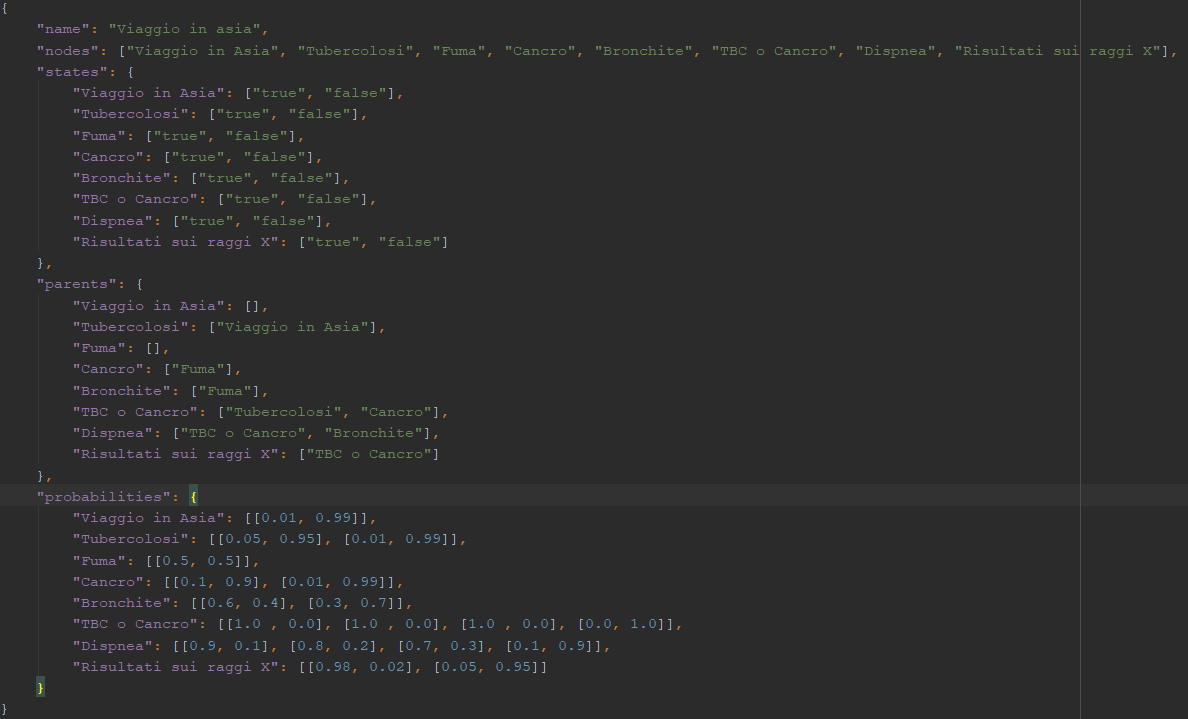
\includegraphics[scale=0.6]{./images/strutturaRete.png}
		 \caption{Rete Bayesiana Correttamente Definita}	
		 \label{ImgRete}
	\end{center}
\end{figure}

Passi da seguire :
\begin{itemize}
 \item Il file \textit{.JSON} dovrà contenere 5 campi più esterni, denominati:
 	\begin{itemize}
 		\item name;
 		\item nodes;
 		\item states;
 		\item parents;
 		\item probabilities.
 	\end{itemize}
 	I nomi dei campi devono iniziare con la lettera minuscola corrispondente. Qualora uno dei campi non abbia il nome corretto come sopra, verrà visualizzato il seguente errore (nel seguente caso mancava il campo name, sostituito da un nome non valido): 
 	\begin{figure}[H]
	\begin{center}
		
\includegraphics[scale=0.6]{./images/erroreNomeCampo.png}
		 \caption{Errore nel Nome di un Campo della Rete Bayesiana}	
		 \label{ImgRete}
	\end{center}
\end{figure}

	Se viene inserito un numero errato di campi diverso da 5, verrà visualizzato il seguente errore:
	
	\begin{figure}[H]
	\begin{center}
		
\includegraphics[scale=0.6]{./images/wrongNumberOfFields.png}
		 \caption{Errore Numero di Campi della Rete Errato}	
		 \label{ImgRete}
	\end{center}
\end{figure}

	\item Il campo successivo dovrà chiamarsi nodes e dovrà contenere un array, nel quale sono definiti i nomi dei nodi della rete bayesiana.\label{nomi} I campi states, parents e probabilities, dovranno ognuno contenere al proprio interno un numero di campi pari al numero di nomi definiti nel campo nodes e con lo stesso nome. Qualora sia definito all'interno di uno di essi un numero errato di campi, verrà visualizzato il seguente errore (ad esempio se manca un nome in states): 

\begin{figure}[H]
	\begin{center}
		
\includegraphics[scale=0.6]{./images/numberFields.png}
		 \caption{Errore Numero di Campi}	
		 \label{erNumCampi}
	\end{center}
\end{figure}

Se invece il numero di campi è giusto ma non viene trovato uno dei nomi in nodes, verrà visualizzato il seguente errore ( il nodo tubercolosi è stato sostituito con un nome non valido):

\begin{figure}[H]
	\begin{center}
		
\includegraphics[scale=0.6]{./images/wrongName.png}
		 \caption{Errore Nome di un Campo Interno}	
		 \label{erNumCampi}
	\end{center}
\end{figure}

	\item Il campo successivo dovrà chiamarsi states e dovrà essere composto nel seguente modo:
	\begin{itemize}
		\item Deve rispettare quanto detto  in \ref{nomi};
		\item Ogni campo dovrà contenere un array con almeno 2 valori al suo interno, altrimenti verrà visualizzato il seguente errore :
		
		\begin{figure}[H]
	\begin{center}
		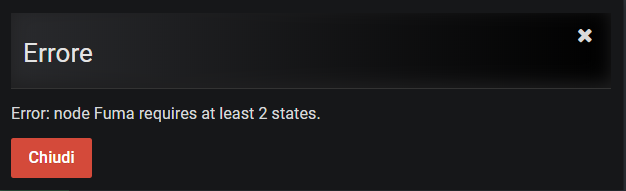
\includegraphics[scale=0.6]{./images/twoStates.png}
		 \caption{Errore Nodo con Meno di 2 Stati}	
		 \label{erTwoStates}
	\end{center}
	\end{figure}
	
		\item Uno stato non può essere ripetuto, altrimenti verrà visualizzato il seguente errore:
	\end{itemize}
	
	\begin{figure}[H]
	\begin{center}
		
\includegraphics[scale=0.6]{./images/multipleState.png}
		 \caption{Errore Stato Ripetuto}	
		 \label{erMultipleState}
	\end{center}
	\end{figure}
	
	\item Il campo successivo dovrà chiamarsi parents e dovrà essere composto nel seguente modo:
	
	\begin{itemize}
		\item Deve rispettare quanto detto  in \ref{nomi};
		\item Ogni campo dovrà contenere un array, nel quale si possono inserire i padri del nodo qualora ne abbia;
		\item I padri devono essere nomi contenuti nel campo nodes, altrimenti verrà visualizzato il seguente errore ( inserito un padre chiamato notValid ):
		
	\begin{figure}[H]
	\begin{center}
		
\includegraphics[scale=0.6]{./images/unexistingNode.png}
		 \caption{Errore Padre non Esistente}	
		 \label{erUnexistingNode}
	\end{center}
	\end{figure}	
	
	\item Un nodo non può essere definito come padre di se stesso, altrimenti verrà visualizzato il seguente errore ( fuma definito come padre di se stesso ):	
	
	\begin{figure}[H]
	\begin{center}
		
\includegraphics[scale=0.6]{./images/padreDiSeStesso.png}
		 \caption{Errore Padre di Sé Stesso}	
		 \label{erUnexistingNode}
	\end{center}
	\end{figure}	
	
	\item Non è possibile definire più volte lo stesso padre per un nodo, altrimenti verrà visualizzato il seguente errore (Fuma definito 2 volte come padre per tubercolosi ): 
	
	\begin{figure}[H]
	\begin{center}
		
\includegraphics[scale=0.6]{./images/padreRipetuto.png}
		 \caption{Errore Padre Ripetuto}	
		 \label{erUnexistingNode}
	\end{center}
	\end{figure}	
		
	\end{itemize}
	
	\item Il campo successivo dovrà chiamarsi probabilities e dovrà essere composto nel seguente modo:
	
	\begin{itemize}
		\item Deve rispettare quanto detto  in \ref{nomi};
		\item Ogni campo deve contenere un array, contenente a sua volta tanti sotto-array pari alla produttoria del numero di stati di ogni padre del nodo, in caso contrario verrà visualizzato il seguente errore(3 al posto di 4):
		
		\begin{figure}[H]
	\begin{center}
		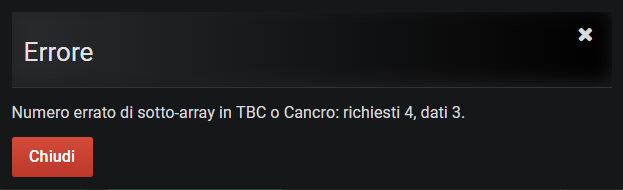
\includegraphics[scale=0.6]{./images/wrongSubsets.png}
		 \caption{Errore Numero di Subset}	
		 \label{erWrongSubsets}
	\end{center}
	\end{figure}	
		
		\item Ogni sotto-array deve contenere un numero di valori pari al numero di stati del nodo, in caso contrario verrà visualizzato il seguente errore(3 al posto di 2): 
		
		\begin{figure}[H]
	\begin{center}
		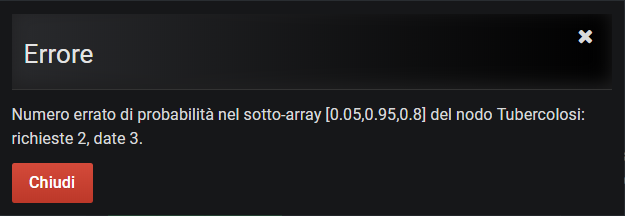
\includegraphics[scale=0.6]{./images/numberProbs.png}
		 \caption{Errore Numero di Probabilità nel Sotto-array}	
		 \label{erWrongSubsets}
	\end{center}
	\end{figure}	
	
	\item Le probabilità devono essere numeri compresi tra 0 e 1, altrimenti verrà visualizzato il seguente errore(probabilità = 5):
	
	\begin{figure}[H]
	\begin{center}
		
\includegraphics[scale=0.6]{./images/invalidProbability.png}
		 \caption{Errore Probabilità non Valida}	
		 \label{erWrongSubsets}
	\end{center}
	\end{figure}
		
	\end{itemize}
	
	\item Le probabilità vanno inserite nel seguente modo:
	 \begin{itemize}
	 		\item in ogni sotto-array le probabilità vanno inserite in ordine in base a come sono stati definiti gli stati del nodo, quindi come in figura \ref{ImgRete} la probabilità 0.01 verrà associata allo stato true e la probabilità 0.99 verrà associata allo stato false;
	 		\item I sotto-array vanno a definire le probabilità condizionate dai padri, e vanno messi in ordine, quindi ad esempio in figura \ref{ImgRete} per il nodo TBC o Cancro, il primo sotto-array andrà a definire le probabilità per p("TBC o Cancro" | Tubercolosi = true, Cancro = true), il secondo p("TBC o Cancro" | Tubercolosi = true, Cancro = false), il terzo p("TBC o Cancro" | Tubercolosi = false, Cancro = true) e l'ultimo p("TBC o Cancro" | Tubercolosi = false, Cancro = false), quindi in ordine secondo come sono stati definiti gli stati dei padri. Nel caso in cui si sbagli a definire i sotto-array, rispettando però i punti precedenti, non verrà visualizzato un errore ma i calcoli non rispetteranno quanto atteso.
	 \end{itemize}
	
	
	
	
	
	
	
	
	

\end{itemize}

\pagebreak

\documentclass[12pt]{article}

\usepackage[utf8]{inputenc}	%Encoding UTF8 per accenti
\usepackage{pdflscape} % per pagine landscape

\usepackage[T1]{fontenc}

\usepackage[italian]{babel}

\usepackage[onehalfspacing]{setspace}	%Interlinea di 1.5

\usepackage[hyperfootnotes=false]{hyperref}	%Pacchetto per coll. ipertestuali

\usepackage{tabularx}
\usepackage{longtable,array} %Per Tabelle potenzialmente multipagina
\usepackage{fancyhdr}  % per gli header e footer
\usepackage{graphicx}  %per le immagini
\usepackage{flafter}
\usepackage{listings} %per i listati di codice
\usepackage[font=small,labelfont=bf]{caption}

\usepackage{framed}

\usepackage[headheight=2cm, headsep=0.5cm, a4paper, margin=3cm]{geometry}
\usepackage[bottom]{footmisc}

\hypersetup{colorlinks=true}		%Configurazione colore link documento
\hypersetup{linkcolor= blue}
\renewcommand\UrlFont{\color{blue}\rmfamily\itshape} %Forzato colore blu su tutti i link ESTERNI

\usepackage[dvipsnames,table]{xcolor}
\definecolor{bluelogo}{HTML}{415A66}
\definecolor{grigio}{HTML}{D0D0D0}
\usepackage{makecell}

\renewcommand{\footrulewidth}{0.1pt}
\newcommand{\glossario}{\textsubscript{G} }

\usepackage{fancyhdr}
\usepackage{lastpage}
 
\pagestyle{fancy}

\fancyhf{}

\lhead{
\includegraphics[scale=0.08]{./images/logo.png}}
\rhead{\rightmark}

\lfoot{Piano di Progetto v2.0.0}
\cfoot{}
\rfoot{Pagina \thepage \hspace{1pt} di \pageref*{LastPage}}

\makeindex
\setcounter{secnumdepth}{4}
\setcounter{tocdepth}{4}

%\lhead{
\includegraphics[scale=0.08]{./images/logo.png}}
%\usepackage[headheight=2cm, headsep=0.5cm, a4paper, margin=3cm]{geometry}

\newcolumntype{C}[1]{>{\centering\arraybackslash}m{#1}}
\usepackage{eurosym}

\usepackage{grffile}
\usepackage{float}



\begin{document}
\begin{titlepage}
\thispagestyle{empty}
\pagenumbering{gobble}

\begin{center}


\includegraphics[scale=0.3]{./images/logo.png} 

\large \textbf{Agents of S.W.E. - Progetto "G\&B"}
\vfill
\Huge \textbf{Glossario}
\vfill
\large
\renewcommand{\arraystretch}{1.3}
\begin{tabular}{r|l}
\textbf{Versione} & 0.0.10\\
\textbf{Approvazione} & ?\\
\textbf{Redazione} & \parbox[t]{5cm}{Luca Violato\\Marco Chilese\\Matteo Slanzi\\Carlotta Segna}\\
\textbf{Verifica} & \parbox[t]{5cm}{?\\?}\\
\textbf{Stato} & Work in Progress\\
\textbf{Uso} & Interno\\
\textbf{Destinato a} & \parbox[t]{5cm}{Agents of S.W.E \\Prof. Tullio Vardanega\\Prof. Riccardo Cardin}
\end{tabular}
\vfill
\small
\texttt{agentsofswe@gmail.com}
\end{center}
\end{titlepage}

\pagebreak

\pagenumbering{Roman}
\tableofcontents
\pagebreak

\pagenumbering{arabic}

\section*{A}
\addcontentsline{toc}{section}{A}

\subsection{\index{Amazon Alexa}Amazon Alexa}
Amazon Alexa è un assistente personale intelligente che, interpretando il linguaggio naturale, è in grado di comunicare con noi. Un’intelligenza artificiale capace di rispondere ai nostri comandi vocali. E'sviluppato dall'azienda Amazon e utilizzato per la prima volta nei dispositivi Amazon Echo e Amazon Echo Dot.

\subsection{\index{Android}Android}
E' un sistema operativo per dispositivi mobili, come smarthphone e tablet, sviluppato da Google e basato su kernel Linux.

\subsection{\index{Apprendimento supervisionato}Apprendimento supervisionato}
E' una tecnica di apprendimento automatico che mira a istruire un sistema informatico in modo da consentirgli di risolvere dei compiti in maniera autonoma sulla base di una serie di esempi ideali, costituiti da coppie di input e di output desiderati, che gli vengono inizialmente forniti.

\subsection{\index{Architettura}Architettura}
Decomposizione organizzata di un sistema in componenti, nonchè l'organizzazione di tali componenti, ovvero la definizione di ruoli, responsabilità e interfacce necessarie all'interazione tra loro stessi.
\section*{B}
\addcontentsline{toc}{section}{B}

\subsection{\index{Best Practice}Best Practice}
Nota metodologia che, secondo l'esperienza professionale o studi autorevoli, abbia mostrato di garantire i migliori risultati in circostanze note e specifiche.
\section*{C}
\addcontentsline{toc}{section}{C}

\subsection{\index{CSS}CSS}

\subsection{\index{CamelCase}CamelCase}
\section*{D}
\addcontentsline{toc}{section}{D}

\subsection{\index{Dashboard}Dashboard}
Nella Software Engineering con tale termine (che letteralmente potrebbe essere tradotto come "Cruscotto") si intente solitamente una pagina  informatica dedicata alla visualizzazione, anche eventualemte storica, di metriche, dati o informazioni, allo scopo di comprendere l'andamento di un progetto.

\subsection{\index{Database}Database}
È una collezione strutturata di dati che hanno una relazione tra loro.

\subsection{\index{DevOps}DevOps}
Acronimo di Development e Operations, DevOps è un approccio allo sviluppo e all’implementazione di applicazioni in azienda, che enfatizza la collaborazione tra il team di sviluppo vero e proprio e quello delle operations, ossia che gestirà le applicazioni dopo il loro rilascio.

\subsection{\index{Diagrammi di Gantt}Diagrammi di Gantt}
Il diagramma di Gantt serve a pianificare un insieme di attività in un certo periodo di tempo. La sua struttura è quella di un semplice diagramma cartesiano in cui le ascisse rappresentano una scala temporale, e le ordinate le cose da fare per portare a termine il progetto. Il tempo per svolgere le attività viene rappresentato con una barra colorata che va dalla data di inizio alla data di fine dell'attività.

\subsection{\index{Digital Ocean}Digital Ocean}
DigitalOcean, è un fornitore di cloud computing americana, fornisce agli sviluppatori servizi cloud che aiutano a distribuire e scalare applicazioni che vengono eseguite simultaneamente su più computer

\subsection{\index{Docker}Docker}
È una piattaforma software che permette di creare build, testare e distribuire applicazioni in tempi brevi. Docker raccoglie il software in unità chiamate container che offrono tutto il necessario per la loro corretta esecuzione.

\subsection{\index{DOM}DOM}
Acronimo di Document Object Model,  è una forma di rappresentazione dei documenti strutturati come modello orientato agli oggetti. Un esempio di albero DOM è quello generato da un browser web nell'interpretazione di un documento HTML.

\subsection{\index{DynamoDB}DynamoDB}
È un servizio di AWS per database non relazionali che offre prestazioni di pochi millisecondi a qualsiasi livello.

\section*{E}
\addcontentsline{toc}{section}{E}

\subsection{\index{ECMA}ECMA}
Acronimo di European Computer Manufacturers Association, è un'associazione fondata nel 1961 e dedicata alla standardizzazione nel settore informatico e dei sistemi di comunicazione. Dal 1994 viene chiamata ECMA International. E' responsabile di molti standard come JSON, ECMAScript.

\subsection{\index{ECMAScript}ECMAScript}
E' un linguaggio di programmazione standardizzato e mantenuto da Ecma International nell'ECMA-262 ed ISO/IEC 16262. Le implementazioni più conosciute di questo linguaggio sono JavaScript, JScript e ActionScript che sono entrati largamente in uso, inizialmente, come linguaggi lato client nello sviluppo web.

\subsection{\index{Efficacia}Efficacia}
Capacità di raggiungere l'obiettivo prefissato, soddisfacendo tutti i suoi requisiti, impliciti ed espliciti.

\subsection{\index{Efficienza}Efficienza}
Misura della capacità di raggiungere l'obiettivo prefissato impiegando le risorse minime indispensabili.

\subsection{\index{ESLint}ESLint}
E' un utility open source per l’analisi statica del codice e per l’identificazione di pattern in JavaScript,  questo permette di trovare più facilmente codice che non rispetta determinate linee guida.
\section*{F}
\addcontentsline{toc}{section}{F}

\subsection{\index{Failure}Failure}
Effetto manifestato da un'esecuzione fallacea.

\subsection{\index{Firebase}Firebase}
È una piattaforma di sviluppo di Google che offre vari servizi tra cui, cloud storage, database realtime in cloud, servizi di autenticazione.

\subsection{\index{Framework}Framework}
Nello sviluppo software, è un'architettura logica di supporto su cui un software può essere progettato e realizzato.

\subsection{\index{FreeLing}FreeLing}
Software open source per l'implementazione di Part of Speech tagger.

\subsection{\index{Front-End}Front-End}
Front-end denota la parte visibile all'utente e con cui può interagire. Di fatto il front-end raccoglie le informazioni e le invia al back-end via una cosiddetta interfaccia, dopo un'opportuna elaborazione dei dati il back-end invierà il risultato al front-end che lo mostrerà all'utente. 
\section*{G}
\addcontentsline{toc}{section}{G}

\subsection{\index{Gamification}Gamification}
Rappresenta uno strumento in grado di veicolare messaggi di vario tipo e di indurre a comportamenti attivi da parte dell’utenza, permettendo di raggiungere specifici obiettivi. Al centro di questo approccio va sempre collocato l'utente ed il suo coinvolgimento attivo.

\subsection{\index{Git}Git}
Software di controllo versione distribuito utilizzabile da interfaccia a riga di comando. Può considerarsi il software di versionamento più diffuso.

\subsection{\index{GitHub}GitHub}
Servizio di hosting per progetti software, è un'implementazione dello strumento di controllo di versionamento Git. Mette a disposizione degli utenti del repository un'interfaccia web per vedere l'albero di directory, i file inseriti e aggiornati e dispone di un sistema di tracciamento delle issue che permette di mantenere una lista delle issue relative al progetto, svolte e da svolgere.

\subsection{\index{GitLab}GitLab}
Come GitHub è un servizio di hosting per progetti software che implementa il controllo di versionamento Git. 

\subsection{\index{Google Drive}Google Drive}
Google Drive è un servizio web, in ambiente cloud computing, di memorizzazione e sincronizzazione online introdotto da Google.

\subsection{\index{Grafana}Grafana}
Piattaforma open source che permette il monitoraggio e l'analisi di dati che vengono visualizzati in dashboard operative. 
\section*{H}
\addcontentsline{toc}{section}{H}
\section*{I}
\addcontentsline{toc}{section}{I}

\subsection{\index{IA}IA}
"Intelligenza Artificiale". Disciplina appartenente all'informatica che studia i fondamenti teorici, le metodologie e le tecniche che consentono la progettazione di sistemi hardware e software
capaci di fornire all'elaboratore elettronico prestazioni, che a un osservatore comune, sembrerebbero essere di pertinenza esclusivamente umana. 

\subsection{\index{Indice di Gulpease}Indice di Gulpease}
Indice di leggibilità di un testo tarato sulla lingua italiana. Si calcola valutando la lunghezza delle parole in lettere, il numero delle parole e il numero delle frasi totali. L'indice risultante è compreso tra 0 e 100: più il valore si avvicina a 100 più il testo è leggibile.

\subsection{\index{InfluxDB}InfluxDB}
InfluxDB è un database ottimizzato per le serie temporali, sviluppato da InfluxData.

\subsection{\index{Issue}Issue}
Problema, attività o compito da svolgere che viene sollevata da un utente, di solito il responsabile, e che viene assegnata oppure auto-assegnata ad un membro del team, può avere una data di scadenza, uno o più tag, una priorità e una breve descrizione.

\subsection{\index{Issue Tracking}Issue Tracking}
Metodo che permette di rintracciare da dove derivano le Issue, a chi sono assegnate, e tracciarne uno storico dello sviluppo.

\subsection{\index{Iterazione}Iterazione}
Atto di ripetere un processo con l'obiettivo di avvicinarsi a un risultato desiderato.


\section*{J}
\addcontentsline{toc}{section}{J}

\subsection{\index{Java}Java}
Linguaggio di programmazione ad alto livello orientato agli oggetti. 

\subsection{\index{JavaScript}JavaScript}
È un linguaggio di scripting orientato agli oggetti, utilizzato nella programmazione web lato client per la creazione di effetti dinamici interattivi, tramite funzioni di script, invocate da eventi innescati dall'utente sulla pagina web.

\subsection{\index{Jest}Jest} 
È un framework di testing di JavaScript. È compatibile con Babel, TypeScript, Node, React, Angular, Vue. Offre la possibilità di eseguire test in parallelo in maniera affidabile, ed eseguire il code coverage di interi progetti.

\subsection{\index{JFrog Artifactory}JFrog Artifactory} 
È un servzio web per la gestione universale di repository.

\subsection{\index{jQuery}jQuery}
Libreria javascript opensource che ha come obiettivo la semplificazione della gestione degli eventi di elementi del DOM in pagine HTML. 

\subsection{\index{Jsbayes}JsBayes}
È una libreria open source per la gestione dei calcoli della rete Bayesiana sviluppata in \textit{JavaScript}.

\subsection{\index{JsbayesViz}JsBayesViz}
È una libreria open source per la visualizzazione delle probabilità delle reti calcolate con \textit{JsBayes}.

\subsection{\index{JSON}JSON}
È un formato utilizzato per il salvataggio e lo scambio di dati in applicazioni client/server.

\subsection{\index{JUnit}JUnit}
È un framework per il linguaggio Java che permette test di unità.
\section*{K}
\addcontentsline{toc}{section}{K}

\subsection{\index{Kotlin}Kotlin}
E' un linguaggio di programmazione utilizzato per lo sviluppo di applicazioni mobile per Android.
\section*{L}
\addcontentsline{toc}{section}{L}
\section*{M}
\addcontentsline{toc}{section}{M}
\section*{N}
\addcontentsline{toc}{section}{N}

\subsection{\index{NodeJS}NodeJS}
Piattaforma open source per scrivere applicazione in JavaScript Server-side.

\subsection{\index{Norme di Progetto}Norme di Progetto}
Documento redatto da un gruppo, interno al gruppo stesso, in cui sono esplicate le regole prefissate da seguire durante tutta la progettazione del prodotto di un dato progetto lavorativo. Tale documento ha come principale contenuto il \textit{"Way of Working"} del gruppo, e risulta essere importante per perseguire economicità e per rendere più efficiente ed efficace la fase di qualifica.

\section*{O}
\addcontentsline{toc}{section}{O}

\subsection{\index{Open Source}Open Source}
Termine utilizzato per indicare programmi software non protetti da copyright. Essenziale per favorire il libero studio e permettere ai programmatori indipendenti di apportarvi modifiche.

\section*{P}
\addcontentsline{toc}{section}{P}

\subsection{\index{Part-of-Speech Tagger}Part-of-Speech Tagger}
È il processo di identificare una parola in un testo come corrispondente a una particolare parte del discorso, in base sia alla sua definizione che al suo contesto, cioè la sua relazione con parole adiacenti e correlate in una frase o paragrafo.

\subsection{\index{Pattern Publisher/Subscriber}Pattern Publisher/Subscriber}
L'espressione publish/subscribe si riferisce a un design pattern o stile architetturale utilizzato per la comunicazione asincrona fra diversi processi, oggetti o altri agenti.

\subsection{\index{PDCA}PDCA}
È un metodo di gestione iterativo in quattro fasi, utilizzato per il controllo e il miglioramento continuo dei processi e dei prodotti.

\subsection{\index{Piano di Progetto}Piano di Progetto}
Documento contenente la pianificazione del lavoro di un gruppo di lavoro per portare a termine un determinato progetto. Esso presenta l'organizzazione delle attività e dei tempi, un preventivo delle risorse necessarie al compimento del progetto, consuntivi di periodo ed analisi di rischi e piani di mitigazione per tali rischi.

\subsection{\index{Piano di Qualifica}Piano di Qualifica}
Documento contente le strategie di verifica e validazione adottate da un gruppo di lavoro per assicurare la qualità di prodotto e di processo in un determinato progetto.

\subsection{\index{Plug-in}Plug-in}
Componente aggiuntivo che interagisce con un altro programma per ampliarne le funzioni.

\subsection{\index{Prodotto}Prodotto}
Output di un processo. In ambito software è un'entità progettata per essere rilasciata all'utilizzatore finale.

\subsection{\index{Product Baseline}Product Baseline}
Presenta la baseline architetturale del prodotto, coerente rispetto a quando riportato nella Technology Baseline. Al suo interno contiene i diagrammi delle classi e di sequenza, la contestualizzazione dei design pattern adottati nell'architettura del prodotto.

\subsection{\index{Progettazione}Progettazione}
Fase del ciclo di vita del software che risponde alla domanda \textit{"Coma va fatta la cosa giusta?"}. È un'attività che, sulla base della specifica dei requisiti prodotta dall'analisi, definisce come tali requisiti debbano essere soddisfatti, ricercando una soluzione soddisfacente per tutti gli stakeholders.

\subsection{\index{Progetto}Progetto}
Insieme di attività e compiti che hanno come proprietà caratteristiche:
\begin{itemize}
	\item Obiettivi Prefissati;
	\item Tempi Fissati, ovvero precise scadenze;
	\item Risorse Limitate che vengono consumate dalle attività di progetto.
\end{itemize}

\subsection{\index{Promise}Promise}
Una \textit{promise} rappresenta un'operazione che non è stata ancora completata, ma che lo sarà in futuro. Gli oggetti \textit{promise} vengono utilizzati per computazioni in differita e asincrone.

\subsection{\index{PoC}Poc}
Vedi \textbf{Proof of Concept}.

\subsection{\index{Proof of Concept}Proof of Concept}
In ambito informatico, consiste nella dimostrazione pratica dei funzionamenti di base di un applicativo o intero sistema.

\subsection{\index{Prototipo}Prototipo}
Modello realizzato nell'ultima fase della progettazione e sperimentazione, e destinato a divenire il punto di partenza della produzione.

\subsection{\index{Pull}Pull}
Comando del sistema di versionamento Git, scarica dal repository remoto tutti i commit effettuati dagli altri membri del team e li applica ai propri file.

\subsection{\index{Push}Push}
Comando del sistema di versionamento Git, permette di inviare al repository remoto le modifiche per cui esiste un commit in locale.

\subsection{\index{Python}Python}
Linguaggio di programmazione ad alto livello.

\section*{Q}
\addcontentsline{toc}{section}{Q}

\subsection{\index{Qualità}Qualità}
Insieme di caratteristiche di un'entità che ne determinano la capacità di soddisfare esigenze espresse e implicite. Tra le più importanti si possono citare: "Conformità ai requisiti", "Idoneità all'uso", "Soddisfazione del cliente".
\section*{R}
\addcontentsline{toc}{section}{R}

\subsection{\index{Repository}Repository}
Struttura che memorizza metadati per un set di file o strutture di directory utilizzato dal sistema di versionamento, centralizzato o distribuito, che è accessibile a più utenti, i quali possono clonare il repository e modificare i file al suo interno per poi reinserirli nel server dove erano presenti.

\subsection{\index{Repository Manager}Repository Manager}
Un proxy per repository remoti che memorizza nella memoria cache gli artefatti risparmiando sia la larghezza di banda che il tempo richiesto per recuperare un artefatto software da un repository remoto.

\subsection{\index{Requisiti}Requisiti}
Capacità che devono essere possedute, oppure condizioni che devono essere soddisfatte, da un sistema per adempiere ad un obbligo.

\subsection{\index{Rete Bayesiana}Rete Bayesiana}
Rappresentazione grafica delle relazioni di dipendenza tra le variabili di un sistema. In statistica la rete bayesiana è utilizzata per individuare più agevolmente le relazioni di dipendenza assoluta e condizionale tra le variabili, al fine di ridurre il numero delle combinazioni delle variabili da analizzare.
\section*{S}
\addcontentsline{toc}{section}{S}

\subsection{\index{Script}Script}
Particolare tipo di programma, scritto con appositi linguaggi interpretati (di scripting per l'appunto), senza interfaccia grafica, aventi solitamente complessità relativamente bassa.

\subsection{\index{Slack}Slack}
Applicazione di messaggistica istantanea, specializzata nella collaborazione aziendale, utilizzata tra i membri del team di lavoro.

\subsection{\index{SonarQube}SonarQube} 
E' uno strumento per la continuous inspection per la qualità del codice.

\subsection{\index{SPICE}SPICE}
Standard ISO/IEC 15504, relativo ad un insieme di documenti tecnici standard per i processi di sviluppo software e le funzioni di gestione di management.

\subsection{\index{SSH}SSH}
E' un protocollo che permette di stabilire una sessione remota cifrata tramite interfaccia a riga di comando con un altro host di una rete informatica.

\subsection{\index{Swift}Swift}
E'un linguaggio di programmazione orientato agli oggetti sviluppato da Apple per sistemi macOS, iOS.

\section*{T}
\addcontentsline{toc}{section}{T}
\section*{U}
\addcontentsline{toc}{section}{U}

\subsection{\index{Use Case}Use Case} 
Tecnica usata nei processi di ingegneria del software per effettuare in maniera esaustiva e non ambigua, la raccolta dei requisiti. Consiste nel valutare ogni requisito focalizzandosi sugli attori che interagiscono col sistema, valutandone le varie interazioni.

\subsection{\index{User-friendly}User-friendly} 
Qualità, solitamente di un prodotto software, che rappresenta l'immediatezza di utilizzo anche per chi non è esperto.

\section*{V}
\addcontentsline{toc}{section}{V}
\section*{W}
\addcontentsline{toc}{section}{W}

\subsection{\index{WireMock}WireMock} 
È un simulatore di HTTP-based API. 
\section*{X}
\addcontentsline{toc}{section}{X}
\section*{Y}
\addcontentsline{toc}{section}{Y}
\section*{Z}
\addcontentsline{toc}{section}{Z}

\subsection{\index{Zeppelin}Zeppelin}
Permette l'analisi tra i dati raccolti ed alcuni linguaggi di programmazione.
\section{Changelog}

\begin{center}
\begin{longtable}[c]{|m{.11\textwidth}|m{.13\textwidth}|m{.1\textwidth}|m{.19\textwidth}|p{.33\textwidth}|}
\hline
\rowcolor{bluelogo}\textbf{\textcolor{white}{Versione}} & \textbf{\textcolor{white}{Data}} & \textbf{\textcolor{white}{Autore}} & \textbf{\textcolor{white}{Ruolo}} & \textbf{\textcolor{white}{Descrizione}}\\
\hline \hline
\endfirsthead
0.0.1 & 2018-11-23 & Luca Violato & Amministratore & Strutturazione del Documento \\
\hline
\rowcolor{grigio} 0.0.2 & 2018-12-18 & Carlotta Segna & Responsabile & Standardizzazione tabella \\
\hline
\caption{Changelog del documento}
\end{longtable}
\end{center}

\pagebreak
\printindex
\addcontentsline{toc}{section}{Indice Analitico}

\end{document}



\end{document}